\chapter{Theoretical Background}\label{chp:theory}

\section{Literature Review}\label{sec:litreview}


The literature review in \Cref{sec:litreview} presents past and present research on the utilisation of machine learning methods to achieve energy-efficient operation. The concept of different modelling approaches for ship operation will be discussed in \Cref{sec:modelling_type}. The summary of the data source in the modelling of FOC is given in \Cref{sec:data_use}. The review of popular machine learning models used to predict FOC is presented in \Cref{sec:ml_var_appl}. The performance of tree-based models, which include random forest and extra trees in various research will be discussed in \Cref{sec:tree_litreview}. Brief summary of the literature review is presented in \Cref{sec:lit_review_conclusion}.\\

\subsection{Modelling Approach for Ship Operation}\label{sec:modelling_type}

According to \bcitet{MichaelHaranen.2016} and \bcitet{Coraddu.2017}, the modelling strategies to predict fuel consumption are classified into three categories:\\

\subsubsection*{\textbf{White Box Models (WBM)}} are based on \emph{a priori} mechanistic knowledge and physical principles of the vessel's system. This means that the dimensions of the vessel's structure, design parameters, and propulsion plant configuration are known.\\

\subsubsection*{\textbf{Black Box Models (BBM)}} are purely data-driven, and it is developed using data from different sailing journeys and historical observations. Contrary to WBM, this approach does not require detailed information on the vessel. This modelling approach can be further split into two categories. \emph{Statistical Modelling} aims to find explanations for relationships between fuel consumption and different factors that affect it. \emph{Machine Learning (ML) Modelling} focuses on the predictive capabilities of the model that could predict fuel consumption at different points in time.\\

\subsubsection*{\textbf{Grey Box Models (GBM)}} fuse WBM and BBM into a single model that considers both \emph{a priori} knowledge of the vessel and historical sailing data, This method aims to complement the performance of WBM and BBM.\\

Each of these strategies possesses its strengths and limitations. WBMs are developed based on physical and hydrodynamics laws, as well as theories of naval architecture. They are transparent and comprehensible, making them the preferred model used by various shipping industries. However, the deterministic nature of WBMs renders them poorly suited for generalisation and adaptability. This limitation arises from the \emph{a priori} knowledge required for vessel dimensions, parameters, and the restricted application scope of principal dimensions and form parameters. Consequently, WBMs' inability to incorporate randomness constrains their flexibility and versatility \bcitet{MichaelHaranen.2016,Yan.2021}.\\

BBMs in general have a good fitting ability for training data and good predictive accuracy for unseen data. BBMs developed using ML approach can generalise better compared to BBMs that are based on statistical modelling \bcitep{Petersen.2012b}. BBMs are purely data-driven, which means BBMs do not require former knowledge of vessel principle dimensions and form parameters. With increasing amounts of data, better generalisation performance and handling of noisy data should be expected in a BBM. However, for the same reason, the quality of BBM model is highly dependent on data quantity and quality. For BBMs based machine learning approach, the amount of data is a major factor in determining the effectiveness of machine learning \bcitep{Halevy.2009}. Data-driven approach means that BBMs neglect basic vessel physical knowledge and are generally complex making it challenging to analyse and explain. For these reasons, experts in shipping industries are critical of models that do not include basic vessel knowledge and those that violate concepts of the domain knowledge in serious ways \bcitep{Yan.2021}.\\   

Hence, GBMs are introduced to address the limitations of both WBMs and BBMs by combining the mechanistic knowledge of the ship and physical principles of the vessel's system with BBM models, which possess good predictive capability. Despite these advantages, \bcitet{Yan.2021} noted that GBM approach is not a common approach, recent research to predict fuel consumption are mainly dominated by BBM approach, specifically BBM based on ML approach.\\

\pagebreak

\subsection{Review of data source used for FOC model}\label{sec:data_use}

The modelling of FOC using GBM requires both components of WBM and BBM. For the BBM modelling part using ML approach, For black-box modelling using ML techniques, it is crucial to have sufficient high-quality data for accurate training \bcitep{Halevy.2009}. \bcitet{Yan.2021} categorise the data sources for FOC modelling as follows:
\\

\subsubsection*{\textbf{(Daily) Noon Report}} These reports are manually prepared by the ship's chief engineer and transmitted by the ship's masters to the shipping company and shore management daily. They contain details about the daily fuel consumption, fundamental voyage particulars (such as the ship's position and load status), sailing behaviour details (such as average sailing speed and average engine RPM), and information about sea and weather conditions. While these reports offer valuable insights into ship operations, the challenge lies in the manual and daily nature of data entry, which can impact both data quality and quantity.\\

\subsubsection*{\textbf{Sensor Data}} Data obtained from onboard installed sensors on the vessel, which might encompass sensors like fuel flow sensors, Global Positioning System (GPS) receivers, and wind speed sensors. These sensors offer a solution to the data quantity issue associated with noon reports, as highlighted in the investigation conducted by \bcitet{Gkerekos.2019} in the context of daily FOC prediction. The machine learning models derived from the Automated Data Logging and Monitoring (ADLM) system demonstrate superior performance compared to models trained using noon data. This improvement amounts to around $5-7\%$ for a data collection span of 3 months using the ADLM system against 2.5 years of noon data. Nevertheless, the implementation of onboard sensors can be intricate and expensive \bcitep{JoanPeturPetersen.2011}, requiring proper management of resulting sensor data to account for potential measurement errors.\\

\subsubsection*{\textbf{AIS Data}} Apart from its primary purpose as a collision avoidance system, AIS data has shown potential for applications in ship behaviour analysis and environmental assessment. The International Maritime Organization (IMO) used AIS data for the study of Greenhouse Gas (GHG) emissions \bcitet{IMO.2020,T.W.P.Smith.2015}, employing it to estimate global shipping emission inventories. \bcitet{Rakke2016} introduced the ECAIS methodology to compute ship emissions based on AIS-derived fuel consumption data. By utilising the Holtrop-Mennen approximation and relevant literature-based approximations, the vessel's propulsion power can be determined, subsequently enabling the prediction of FOC. \bcitet{Kim.2020b} employed publicly accessible AIS data, ship static information, and environmental data, to estimate the Energy Efficiency Operational Indicator (EEOI) by using big data technology. In essence, research utilizing AIS data is directed at achieving independence from reliance on commercial databases. Further elaboration on AIS data can be found in \Cref{sec:ais_theo}.  

\subsection{Review of ML approach to predict FOC}\label{sec:ml_var_appl}

Modelling of FOC using \emph{machine learning} approach generally focus on the prediction of unseen data. The general framework usually includes the collection and preprocessing of ship operational data, training and validation of the model, and evaluation and selection of the most appropriate model. Some machine learning models allow further hyperparameter tuning of the model and in the case of a data-rich environment, the data can be further split into test data to further validate the performance of machine learning model.\\

The study by \bcitet{Yan.2021} indicated that the majority of recent research that uses machine learning approach employs Artificial Neural Network (ANN) as the model to predict FOC. ANN models are powerful models capable of modelling nonlinear data which are based on theories on how the brain works. The outcome is modelled by an intermediate set of unobserved variables known as hidden layer. \bcitep{Kuhn.2013}. Backpropagation neural networks, Multi Level Perceptron (MLP), and wavelet neural networks are some examples of ANN model subclasses.\\

ANN has shown notable performance in its attempt to predict FOC. \bcitet{Petersen.2012} reported Root Mean Square Error (RMSE) of $47.2$ L/h for for fuel flow (FOC) prediction. To provide context, the fuel flow in their case study fluctuates between $1000 - 2500$ L/h. \bcitet{BalBesikci.2016} considered sailing speed, trim, wind, sea effects, propeller pitch, and engine rotation speed as input variables to predict FOC per hour, achieving model fit score of $R^2 = 0.759$ in the test set. Similar ranges of results have been reported in other studies utilising ANNs \bcitep{Yan.2021}.\\

However, the development of ANN models is a challenging task. These models tend to overfit in situations where data availability is limited. Therefore, regularisation is necessary to improve model performance. The balancing process during regularisation is an intricate task and unsuitable regularisation may lead to counterintuitive prediction results. Furthermore, the process of adding layers is computationally resource-expensive and does not always guarantee promising results \bcitep{Hastie.2009}. Moreover, from ML perspective, ANN is classified as a black box model, which makes it unintuitive and lacking in interpretability  \bcitep{Geron.2019}, this particular limitation cause shipping industry expert generally reluctant to accept the model generated using ML approach. \\

\subsection{Tree-Based Model as FOC model}\label{sec:tree_litreview}

Concerning interpretability, modelling approaches such Linear Regression (LR), k-Nearest Neighbour (KNN) and tree-based models have shown superior interpretability in comparison to ANNs. LR can explain the effect of each input variable on the output through the coefficients. KNN searches for the nearest neighbour and their closeness is evaluated through distance measurement algorithms such as Euclidean distance. Additionally, LRs and KNNs also offer easy implementation and adequate explainability. However, both approaches suffer from sensitivity to outliers and noise in data.\\

This brings us to the tree-based model, a supervised, highly interpretable machine learning modelling approach capable of performing classification tasks for discrete data and regression tasks for continuous data. According to the summary of \bcitet{Yan.2021}, it is not as popular as ANN, however, some literature work and studies have indicated its benefits and performance superiority over other machine learning modelling approaches:\\

\bcitet{Soner.2018} used the ferry dataset from \bcitet{Petersen.2012} to predict FOC using tree-based model, which includes bagging, random forest (RF), and bootstrap. From the test dataset, the random forest model achieved RMSE of $43.5$ L/h for the fuel consumption. Which suggested improvement from ANN model from the study of \bcitet{Petersen.2012}.\\ 

\bcitet{Yan.2020} used random forest (RF) model to predict FOC for a voyage of a dry bulk ship using ship operational data i.e. ship noon data and sea and weather data from noon report and ECMWF. The prediction model considered ship sailing speed, total cargo weight and meteorological conditions and the RF model obtained mean absolute percentage error (MAPE) of $7.91\%$ for the FOC prediction. The RF model displayed superior results in comparison to Decision Tree Regressor (DTR), ANN, LASSO, and SVR.\\      

The advantage of tree-based model is further highlighted by \bcitet{Gkerekos.2019}. The study compared the performance of different machine learning models to predict ship's FOC per day using both noon data and automated data logging and monitoring (ADLM) system from a bulk carrier. This research concludes that tree-based model displayed good prediction performance on both noon data and sensor-based data. ETR achieved remarkable model fit score of $89\%$ using the noon data and $97\%$ when using the data from ADLM system, outperforming ANN, SVR, and RFR models.\\

\bcitet{Li.2022} performed more extensive research on the effects of data fusions between meteorological data, ship voyage data, and AIS data on different machine learning models to predict the ship's FOC. The study classified ETR and RFR as tree-based model which is produced by \emph{bagging ensemble strategy}. While AdaBoost (AB), Gradient Tree Boosting (GB), XGBoost(XG) and LightGBM (LB) are classified as tree-based models produced by \emph{boosting ensemble strategy}. The study recommends all tree-based models that are produced by \emph{boosting ensemble strategy} and ETR to be used to model energy efficient operation. Additionally, RFR shows the best robustness among the proposed model in the study.\\

\bcitet{Abebe.2020} attempted to use ML approach to predict SOG of the ship. In this study, AIS data and noon-report weather data from 14 tracks and 62 ships are used for model training. The model considered the ship draught, ship dynamic information, tonnage, and environmental conditions. The result of this study exhibited the feasibility of using AIS data and meteorological data to predict SOG of the ship. The results also further indicated the strength of the tree-based model, on the test dataset, ETR achieved the best result with $R^2$ score of $98.47\%$ and RMSE of $0,234$ knots. It is also reported that ETR achieved better performance with about half of the computational cost of RFR.\\ 

\subsection{Review of WBM for FOC prediction}\label{sec:wbm_review}

To predict the FOC of a ship, WBMs usually calculate the resistances encountered by the vessel based on physics and hydrodynamic laws. The total resistance is cumulated from calm water resistance and additional resistance from wind, wave, and other external factors. This, in turn, allows for the determination of the corresponding engine power at a given speed which allows the calculation of the FOC \bcitep{MichaelHaranen.2016}.\\

The methods from \bcitet{Guldhammer.1974}, \bcitet{Hollenbach.1999}, and \bcitet{Kristensen.2012} use different formulations, assumptions, and input variables for engine power estimation. For this thesis, the main focus will be the use of the estimation method from Holtrop-Mennen \bcitep{Holtrop.1978,Holtrop.1982,Holtrop.1984}. Holtrop-Mennen estimate method allowable application range is suitable in most cases. This is indicated by studies from \bcitet{Rakke2016} and \bcitet{Kim.2020b}. \bcitet{Rakke2016} used ship operational and mechanical data from various works of literature and AIS data for input variables to estimate the engine power using Holtrop-Mennen method to subsequently calculate FOC. The FOC is then used to estimate GHG emissions for different ships and the study reported about $5\%$ error rate during model testing. \bcitet{Kim.2020b} successfully estimated Energy Efficiency Operational Index (EEOI) without actual FOC. The study used AIS data as well as publicly accessible weather data and ship static information. The approach in this study used Holtrop-Mennen method to estimate engine power which is consequently used to calculate FOC for EEOI estimations.\\ 

\subsection{Conclusion of Literature Review}\label{sec:lit_review_conclusion}

As categorised by \bcitet{Yan.2021}, the GBM model in this thesis falls under the category of sequential GBM, Here, the BBM and the WBM are sequentially developed and then combined to form the GBM. The BBM is designed for predictions of unseen data, and its outcomes are subsequently fed into the WBM. The use of the tree-based ML model addresses the challenge of limited interpretability faced by certain machine learning models. Furthermore, tree-based models can outperform most of the available machine learning models while providing added benefits of little requirement for data preprocessing and relatively cheap computational cost. The selection of Holtrop-Mennen as energy estimation method is justified by the application range of the methodology and reported successes in prior studies.\\ 

\section{Tree-based model}\label{sec:tree_intro}

Decision Tree, Random Forest and Extra-Tree are classified as tree-based model, which is supervised machine learning model capable of classification tasks for discrete variables and regression tasks for continuous variables. In this section, the theory of Decision Tree (DT), Random Forest (RF) and Extra Tree (ET) will be discussed in detail in \Cref{sec:dt_theo}, \Cref{sec:rf_theo} and \Cref{sec:et_theo}.\\  

\subsection{Decision Tree}\label{sec:dt_theo}

The principle of decision tree as a predictor can be defined as one or more nested {\tt if-then} statements based on a rule that partitions the data into partition space as shown in \Cref{fig:partitionspace}. Alternatively, the partition space formed through {\tt if-then} statements can also be visualised using a binary tree representation, which offers greater interpretability since various input responses can be represented through a single tree \bcitep{Kuhn.2013, Hastie.2009}.\\

A decision tree consists of the following type of nodes, \textbf{\emph{Root node}} defines the topmost node. \textbf{\emph{Leaf nodes}} are also termed as terminal nodes, it is the node that will give the final prediction output. The \textbf{\emph{Internal Node}} is defined as the nodes between the root node and leaf node. The process of dividing a node into successive nodes is called \textbf{\emph{splitting}}. The node that is being split is called \textbf{\emph{parent node}} and the successive nodes that are created are called \textbf{\emph{child nodes}}. To grow a tree in a regression task, the splitting process is typically regulated by Mean Square Error (MSE). The tree growth algorithm is based on Classification and Regression Tree (CART).\\

To understand the principle of selection for the feature, $\text{k}_t$ , of the parent node and splitting rule, $\text{t}_k$ , for data partition, the following example will be presented:\\

\begin{figure}
\centering
\begin{minipage}[b]{.5\textwidth}
    \centering
    \begin{tikzpicture}[x=0.75pt,y=0.75pt,yscale=-1,xscale=1]
    %uncomment if require: \path (0,433); %set diagram left start at 0, and has height of 433
    
    %Shape: Square [id:dp5731268858272198] 
    \draw   (180,110) -- (370,110) -- (370,300) -- (180,300) -- cycle ;
    %Straight Lines [id:da615072570759449] 
    \draw    (250,110) -- (250,300) ;
    %Straight Lines [id:da8002566967918264] 
    \draw    (300,110) -- (300,300) ;
    %Straight Lines [id:da4409034763483005] 
    \draw    (180,230) -- (250,230) ;
    %Straight Lines [id:da07514682530914596] 
    \draw    (300,170) -- (370,170) ;
    
    % Text Node
    \draw (131,192.4) node [anchor=north west][inner sep=0.75pt]    {$X_{2}$};
    % Text Node
    \draw (261,340.4) node [anchor=north west][inner sep=0.75pt]    {$X_{1}$};
    % Text Node
    \draw (157,222.4) node [anchor=north west][inner sep=0.75pt]    {$t_{2}$};
    % Text Node
    \draw (201,252.4) node [anchor=north west][inner sep=0.75pt]    {$R_{1}$};
    % Text Node
    \draw (201,162.4) node [anchor=north west][inner sep=0.75pt]    {$R_{2}$};
    % Text Node
    \draw (268,192.4) node [anchor=north west][inner sep=0.75pt]    {$R_{3}$};
    % Text Node
    \draw (321,132.4) node [anchor=north west][inner sep=0.75pt]    {$R_{4}$};
    % Text Node
    \draw (321,220.4) node [anchor=north west][inner sep=0.75pt]    {$R_{5}$};
    % Text Node
    \draw (241,310.4) node [anchor=north west][inner sep=0.75pt]    {$t_{1}$};
    % Text Node
    \draw (291,312.4) node [anchor=north west][inner sep=0.75pt]    {$t_{3}$};
    % Text Node
    \draw (381,162.4) node [anchor=north west][inner sep=0.75pt]    {$t_{4}$};
    
    \end{tikzpicture}
    
    \captionof{figure}{Example of partition space \bcitep{Hastie.2009}} 
    \label{fig:partitionspace}
\end{minipage}%
\begin{minipage}[b]{.5\textwidth}
    \centering
    \begin{tikzpicture}
        \tikzset{level distance=65pt,sibling distance=10pt,edge from parent/.style=
        {draw,edge from parent path={(\tikzparentnode.south)
                                -- +(0,-8pt)
                                -| (\tikzchildnode)}}}
    \Tree [.$X_1\leq t_1$ [.$X_2\leq t_2$ [.$R_1$ ] [.$R_2$ ] ]
        [.$X_1\leq t_3$ [.$R_3$ ]
        [.$X_2\leq t_4$ [.$R_4$ ] [.$R_5$ ] ] ] ]
    \end{tikzpicture}
    \captionof{figure}{Example of partition tree \bcitep{Hastie.2009}} 
    \label{fig:partitiontree}
\end{minipage}
\end{figure}

\textbf{For the selection of the optimal splitting rule $t_k$}: Given a case with single feature $\text{k}$ and response $y$ with $n$ data points present. The algorithm starts by looking for possible splits between two distinct data points $y$. This split results in two distinct partition spaces. For each partition space $\text{S}_1$ and $\text{S}_2$, the mean is calculated by dividing the sum of response $y$ with the amount of data points $n$ for each respective partition space $\text{S}_1$ and $\text{S}_2$.\\ 

This step is then followed by calculating the sum of squared error (SSE) of each data point in partition space $\text{S}_1$ and $\text{S}_2$, followed by division by the respective numbers of data points, $n{\text{S}1}$ and $n{\text{S}_2}$, to calculate the mean sqaured error (MSE). Next, the MSE values from the partition spaces $\text{S}_1$ and $\text{S}_2$ are aggregated. This iterative process continues recursively until a threshold $\text{t}_k$ is identified. which yields the minimum sum of MSE, this threshold will be selected as splitting rule for the parent node and correspond to the threshold that minimises the cost function $J(\text{k},\text{t}_k)$, Here, $\hat{y}{\text{S}i}$ represents the mean of the response variable $y{\text{S}_i}$ within the partition space $\text{S}_i$. \bcitep{Geron.2019,Kuhn.2013}.

\begin{equation}\label{eqn:sse}
    \text{MSE}_{\text{S}_i} = \frac{1}{n_{\text{S}_i}}\text{SSE}_{\text{S}_i} \quad \textbf{where} \quad i = (1,2)   
\end{equation}
\begin{equation}\label{eqn:costfun}
    J(\text{k},\text{t}_k) = \frac{1}{n_{\text{S}_1}}\text{SSE}_{\text{S}_1} + \frac{1}{n_{\text{S}_2}}\text{SSE}_{\text{S}_2}
    \begin{cases}
        \text{SSE}_{\text{S}_i} = \sum\limits_{i \in \text{S}_i}(\hat{y}_{\text{S}_i} - y_{\text{S}_i} )^2 \\
        \hat{y}_{\text{S}_i} = \frac{1}{n_{\text{S}_i}}\sum\limits_{i\in \text{S}_i} y
    \end{cases}  
\end{equation}

\textbf{For the selection of the most optimal feature for parent node $\text{t}_k$}: Similar principle is also applied for the selection of the most optimal feature for the parent node. Consider there are $\text{k}_t$ features, then for each respective feature $\text{k}_1,\text{k}_2,\dots,\text{k}_t$, The MSE for each of the features is calculated following the cost function $J(\text{k},\text{t}_k)$. The feature that can best \emph{\textbf{minimise}} the cost function will be selected as the root node of the tree. The subsequent selections of the feature for the parent node follow the same principle. \bcitep{Hastie.2009,Geron.2019}.\\

After this step, the partition space is subsequently divided into two additional regions in order to identify the next potential split that minimizes the cost function $J(\text{k},\text{t}_k)$. This recursive process continues until either the number of samples for splitting reaches a predefined threshold or when no further split can be found which reduces the MSE.\\


\begin{figure}[h]
    \centering
    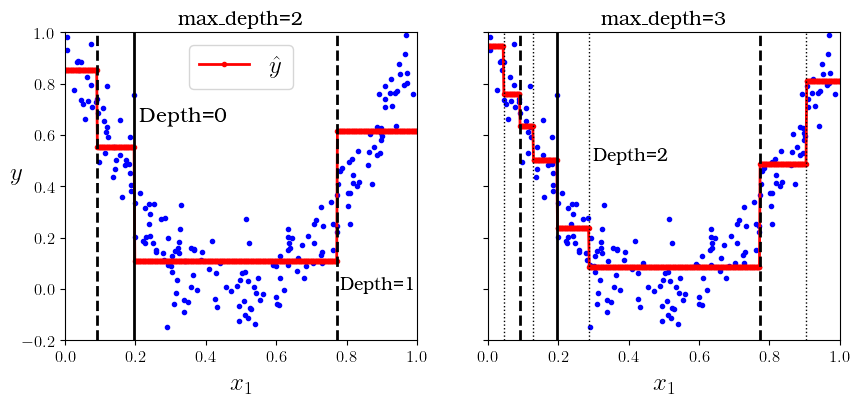
\includegraphics[width=.9\textwidth]{02_figures/fig6_5_partspace_geron09.png}
    \caption{Prediction of two Decision tree regression models \bcitep{Geron.2019}}
    \label{fig:geron6_5}
\end{figure}

The resulting decisions for the best possible splits can be represented using binary tree, this makes decision tree highly interpretable and easy to implement. The inherent logic structure from {\tt if-then} statements means that it can handle various types of data (sparse, skewed, continuous, categorical, etc.) without the need for data pre-processing. Decision tree implicitly conducts feature selection which is a desirable trait for many modelling problems \bcitep{Kuhn.2013}.\\

However, a single decision tree suffers from overfitting when the model is unconstrained. The logical principle of {\tt if-then} statements means that decision tree will attempt to fit the training data as closely as possible. Furthermore, a single decision tree model tends to be unstable, altering the data will cause drastic changes in the structure of the tree, there exist possibilities where completely different sets of splits might be found resulting in different interpretations \bcitep{Hastie.2009,Kuhn.2013}. From \Cref{fig:partitionspace}, it can be implied that each decision boundaries are orthogonal to an axis i.e. all splits are perpendicular to an axis and this form rectangular subspaces for each predicted value. If the relationship between predictors and response cannot be adequately defined by the rectangular subspaces, then tree-based models will suffer from larger prediction errors than other kinds of models \bcitep{Kuhn.2013}.\\

Therefore, it is necessary to regularise i.e., restrict the decision tree's freedom to grow during model training. Overfitting could be reduced by controlling how deep the tree can grow through the {\tt max\_depth} parameter. Additionally, setting the amount of minimum number of samples a leaf node has, through {\tt min\_samples\_leaf} can alleviate overfitting as well, as shown in \Cref{fig:geron6_6}. Other regularisation techniques will be discussed in \Cref{sec:hpo}. Regularisation may result in better generalisation capability. Nonetheless, in order to attain significant improvements in the performance of the decision tree model, it is necessary to seek alternative solutions.\\

\begin{figure}
    \centering
        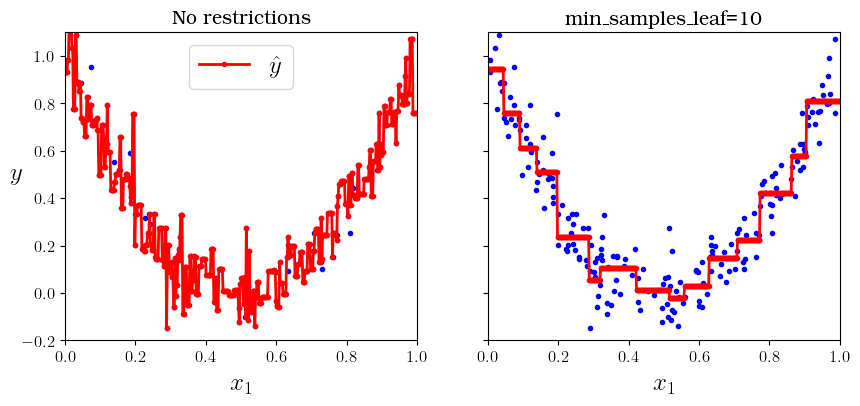
\includegraphics[width=.9\textwidth]{02_figures/fig6_6_paramdepth_geron09.png}
        \caption{Regularising a Decision Tree regressor \bcitep{Geron.2019}}
        \label{fig:geron6_6}
\end{figure}

\subsection{Random Forest}\label{sec:rf_theo}

Ensemble learning is one of the possible solutions to improve the performance of DT regressors. The main idea of ensemble learning is combining the strengths of a collection of simpler base models \bcitep{Hastie.2009}. The algorithm, involving the creation of bootstrap samples, random selection of splitting feature and aggregation of the prediction is termed by \bcitet{Breiman.2001} as \textbf{\emph{Random Forest}}. It involves the combination of multiple learning algorithms, known as weak learners, where each of these learners corresponds to an individual decision tree in the case of Random Forest.

The most common ensemble methods are \emph{boosting} and \emph{bagging}. In boosting, the learner evolves, where successive trees are dependent on the earlier trees. In bagging (short for \emph{bootstrap aggregating}) each tree is trained using bootstrap sample of the training set i.e. this means that a sample of the training dataset is randomly selected and allowed to appear more than once\footnote{This sampling technique is referred to as sampling \emph{with} replacement}. Each model in the ensemble then generates a prediction from the bootstrapped sample and the predictions are aggregated across the learners \bcitep{TinKamHo.1995,Breiman.2001}.\\

The performance of bagging can be further improved by reducing the correlation between trees i.e. de-correlating trees. This can be achieved by adding randomness during the tree construction process. \bcitet{Dietterich.2000} introduced the idea of random split selection, which means that a feature k will be selected from a random subset of features. From this random subset, the assignment of the feature for the parent node follows the CART algorithm described in \Cref{eqn:costfun}. Further randomness is added by exploiting the instability of a single decision tree mentioned in \Cref{sec:dt_theo}.\\

The methodology introduced in random forest address the tendency of decision tree to overfit and the issue of lack of robustness. De-correlating trees means that each learner is independent of the other, and the combination of many independent, strong learners yields an improvement in error rates i.e. reduction in variance and robustness against noisy response. It is also proven by \bcitet{Breiman.2001} that random forest cannot overfit, which means growing more trees should not affect the performance of random forest, albeit with a greater computational burden. Both \bcitet{Kuhn.2013} and \bcitet{Hastie.2009} reported that remarkable prediction results can be obtained without extensive tuning of tree parameters. \\

However, random forest loses the benefit of interpretability of basic tree-based model. While it remains feasible to trace the path within an individual tree to comprehend the decisions leading to a particular prediction, the ensemble nature of random forest hinders the possibility to gain an understanding between the feature and the prediction. Nevertheless, it is still possible to quantify the impact of each feature in the ensemble \bcitep{Kuhn.2013}\footnote{Known as feature importances in \scikit/}. Random forest also tends to perform poorly with a small number of samples \bcitep{Hastie.2009}.\\

\subsection{Extra-Trees (Extremely Randomised Trees)}\label{sec:et_theo}

Extra-trees (Extremely Randomised Trees) was introduced by \bcitet{Geurts.2006} to further randomise random forest and further de-correlate the trees in the forest. Unlike random forest, which selects the optimal split by selecting the best feature among randomly selected subset of features, Extra-trees selects a split at random. Extra-trees also does not bootstrap the sample\footnote{This sampling technique is referred to as sampling \emph{without} replacement} and uses the whole training dataset. The random selection of split means that it saves computational power and the increase in variance caused by tree de-correlation can be countered by increasing the number of trees in the ensemble.\\ 

\pagebreak

\section{AIS Data}\label{sec:ais_theo}

\subsection{Overview of AIS}

Automatic Identification System (AIS) is an automated tracking system onboard ships that was developed automatically transmit information about the ship to other ships and coastal authorities to avoid ship collision accidents. As part of the revised new chapter V of SOLAS\footnote{International Convention for the Safety of Lives at Sea} regulation, International Maritime Organization (IMO) requires all international voyage ships of 300 gross tonnage (GT) and upwards, cargo ships with 500 GT not engaged on international voyage, and all passenger ships irrespective of size to be equipped of AIS class A equipment \bcitep{Yang.2019,webimo.2014}.\\

AIS uses Very High Frequency (VHF) with special protocol for communication system for information exchange between the ships. This information will be received by ships directly, buoys, Land-based (terrestrial) AIS transceivers (T-AIS) and satellites (S-AIS). The information transmitted by AIS is distinguished into three different types. \textbf{Static information} which is entered into the AIS on installation, \textbf{dynamic information}, which is automatically updated from the ship's sensors connected to AIS and \textbf{voyage-related information}, which might required manual entry and updating during the voyage. The structure of the AIS data that is relevant to this thesis is summarised in \Cref{tbl:AIS_struct}\bcitep{webimo.2014}.\\

AIS is also further differentiated by its equipment class. The classification is based on the reporting interval and the type of information that is conveyed. \textbf{Class A} autonomously report their position within 2-10 seconds intervals, depending on the state of the ship's movement. The reporting interval is less frequent, occurring every 3 minutes, particularly when the ship is at anchor, moored, or moving at a speed slower than 3 knots. \textbf{Class A AIS} is also equipped to transmit safety-related information, meteorological and hydrological data, electronic broadcasts to mariners, and marine safety messages.  On the other hand, \textbf{Class B AIS} reports at longer intervals and with lower power. Class B AIS can only receive safety-related messages and is not capable of sending them. \bcitet{Rakke2016, webimo.2014}

\begin{table}[h!]
    \footnotesize
    \centering
    % \resizebox {\textwidth}{!}
    {\begin{tabular}{ p{0.27\linewidth} p{0.67\linewidth}  }
    \hline
    \textbf{Information Item} & \textbf{Description} \\
    \hline
    \multicolumn{2}{l}{\textbf{Static}}\\
    \hline
    MMSI & MMSI number of vessel\\
    Callsign & Callsign of vessel \\
    Name & Name of the vessel \\
    IMO & IMO number of the vessel \\
    Length & Length of vessel \\
    Width & Width of vessel \\
    Ship Type & Describes the AIS ship type of this vessel \\
    \hline
    \multicolumn{2}{l}{\textbf{Dynamic}}\\
    \hline
    Ship's position & Automatically updated from position sensor connected to AIS. Longitude and Latitude.\\
    Position time stamp in UTC & Automatically updated from ship's main position sensor. Format: DD\slash MM\slash YYYY HH:MM:SS\\
    Course over Ground (COG) & \emph{\textbf{If available}}, automatically updated from ship's main position sensor connected to AIS.\\  
    Speed Over Ground (SOG) & \emph{\textbf{If available}}, automatically updated from the position sensor connected to AIS.\\
    Heading & Automatically updated from the ship's heading sensor connected to AIS\\
    Navigational status & Navigational status information has to be manually entered by the Officer on Watch (OOW) and changed as necessary. For example : ``\emph{underway by engines}'',``\emph{engaged in fishing}'',``\emph{at anchor}''.\\
    Rate of Turn (ROT) & \emph{\textbf{If available}}, Automatically updated from the ship's ROT sensor or derived from
    the gyro.\\
    \hline
    \multicolumn{2}{l}{\textbf{Voyage Related}}\\
    \hline
    Ship's draught & To be manually entered at the start of the voyage using the maximum draft for the voyage and amended as required \\
    Cargo Type & Type of (hazardous) cargo from AIS message.\\
    Destination and ETA & To be manually entered at the start of the voyage and kept up to
    date as necessary.\\
    \hline
    \end{tabular}}
\caption{Structure of AIS data \bcitep{webimo.2014}}\label{tbl:AIS_struct}
\end{table}

\pagebreak

It is also stated by \bcitet{Yang.2019} that AIS data can be combined with data from other databases to provide additional information such as:\\

\begin{itemize}
    \setlength\itemsep{0em}
    \item Port-to-port average speed: the voyage time can be calculated from the time stamps reported by AIS data; the voyage distance can be found from corresponding navigation distance tables.
    \item Cargo weight which can be estimated from draught and ship size.
    \item Technical ship specification from fleet database which can be derived from IMO number.
    \item Port-to-port bunker consumption which can be estimated based on the speed, technical ship specification and distance between two ports.
\end{itemize}

\subsection{Speed Correction}\label{sec:SOG_corr}

The speed displayed in AIS represents the speed over ground (SOG). However, to calculate bunker fuel consumption, the ship's actual speed, known as speed through water (STW), is required. Therefore, a correction needs to be applied to SOG to obtain STW. This correction is carried out by considering the current speed $v_C$ and the current direction $\gamma$ \emph{with respect to True North}. In principle, STW will be greater than SOG when the ship is moving against the current, as the ship needs to compensate for the current to maintain the SOG. Conversely, STW will be less than SOG when the ship is moving in the same direction as the current.\\

To calculate the correction, this study will adopt the methodology proposed by Kim et al. \bcitep{Kim.2020b} and Yang et al. \bcitep{Yang.2020}. The $x$ and $y$ components of SOG can be obtained through vector decomposition using the ship's heading angle $\alpha$ \emph{with respect to True North}. Similar vector decomposition is also performed for current speed $v_{\text{C}}$, it is resolved with current direction $\gamma$ \emph{with respect to True North}:\\

\begin{equation}\label{eqn:sogx}
    v_{\text{G}}^x = v_{\text{G}}\cdot\sin(\alpha)   
\end{equation}
\begin{equation}\label{eqn:sogy}
    v_{\text{G}}^y = v_{\text{G}}\cdot\cos(\alpha)   
\end{equation} 
\begin{equation}\label{eqn:vcurrx}
     v_{\text{C}}^x = v_{\text{C}}\cdot\sin(\gamma)   
\end{equation}
\begin{equation}\label{eqn:vcurry}
    v_{\text{C}}^y = v_{\text{C}}\cdot\cos(\gamma)   
\end{equation}

Then the resulting equation to determine STW,$v_{\text{S}}$, including the current compensation, is given by:\\

\begin{equation}\label{eqn:stwx}
    v_{\text{S}}^x = v_{\text{G}}^x - v_{\text{C}}^x    
\end{equation}
\begin{equation}\label{eqn:stwy}
    v_{\text{S}}^y = v_{\text{G}}^y - v_{\text{C}}^y      
\end{equation}
\begin{equation}\label{eqn:stwabs}
    v_{\text{S}} = \sqrt{(v_{\text{S}}^x)^2 + (v_{\text{S}}^y)^2} 
\end{equation}

\subsection{Source of error in AIS}\label{sec:AIS_error}

AIS data may still contain errors and inaccuracies. Manual data entry, particularly for static information and voyage-related details such as estimated time of arrival (ETA) and draught, is a primary source of errors. Instances have been observed where the Maritime Mobile Service Identity (MMSI) is shared by different ships, despite its intended uniqueness. Furthermore, data collected automatically by sensors can also be erroneous, which may arise from sensor malfunctions or improper installations \bcitep{Yang.2019}. Therefore, it is necessary to preprocess the AIS data to ensure an accurate representation of the ship's state during her voyage.\\    

\section{Weather data}\label{sec:weather_theo}

Throughout a voyage, a vessel can encounter winds and waves originating from different directions and with varying magnitudes. These atmospheric and hydrodynamic factors can influence the vessel's trajectory during the journey, impact vessel performance elements like speed and engine power, and even affect a vessel's ability to navigate challenging sea conditions i.e. a vessel's seakeeping capabilities \bcitep{Molland.2011}. To ensure an accurate estimation of the engine power needed by the vessel, it is important to account for different weather conditions. Therefore, this section will primarily focus on the definition of wind and wave effects and explore the interrelation between some of these key parameters.\\ 

\subsection{Definitions of weather parameters}\label{sec:weather_definition}

\subsubsection*{Wind Waves and Swell}

\textbf{Wind Waves} are also known as wind sea, wind waves are irregular and short-crested waves generated by local wind. \textbf{Swell} are waves that travel outside the wave generation area and are no longer the result of wind, they take on regular and long-crested appearance \bcitep{Holthuijsen.2007}

\subsubsection*{Significant Wave Height, $H_{1/3}$}

It is defined as the mean of the highest one-third of waves in the wave record. The distribution of wave heights can be represented by probability density function. Hence, the term ``highest one-third of waves'' here means the region of wave heights that belong in the upper one-third of a probability density function, this is illustrated in \Cref{fig:wavestats}. From this distribution, the relation between significant wave height $H_{1/3}$, the highest ten percent of waves $H_{10}$, maximum wave height $H_{max}$ and average wave height $\overline{H}$ can be summarised as follows \bcitep{bretschneider.1965,Holthuijsen.2007}: 
\begin{equation}\label{eqn:Hsig_mean}
    \overline{H} = 0.625\cdot H_{1/3}
\end{equation}
\begin{equation}\label{eqn:Hsig_Hten}
    H_{10} = 2.03\cdot \overline{H} = 1.27\cdot H_{1/3} 
\end{equation}
\begin{equation}\label{eqn:Hsig_max}
    H_{\text{max}} = 2 \cdot H_{1/3} 
\end{equation} 

Additionally, \bcitet{BitnerGregersen.2005} and \bcitet{Nielsen.2020} described the relation between the significant wave height, wind wave height and swell height through the following equation:

\begin{equation}\label{eqn:H_sig_root}
    H_{1/3} = \sqrt{(H_{\text{swell}})^2 + (H_{\text{windwave}})^2} 
\end{equation}

\begin{figure}[h]
    \centering
        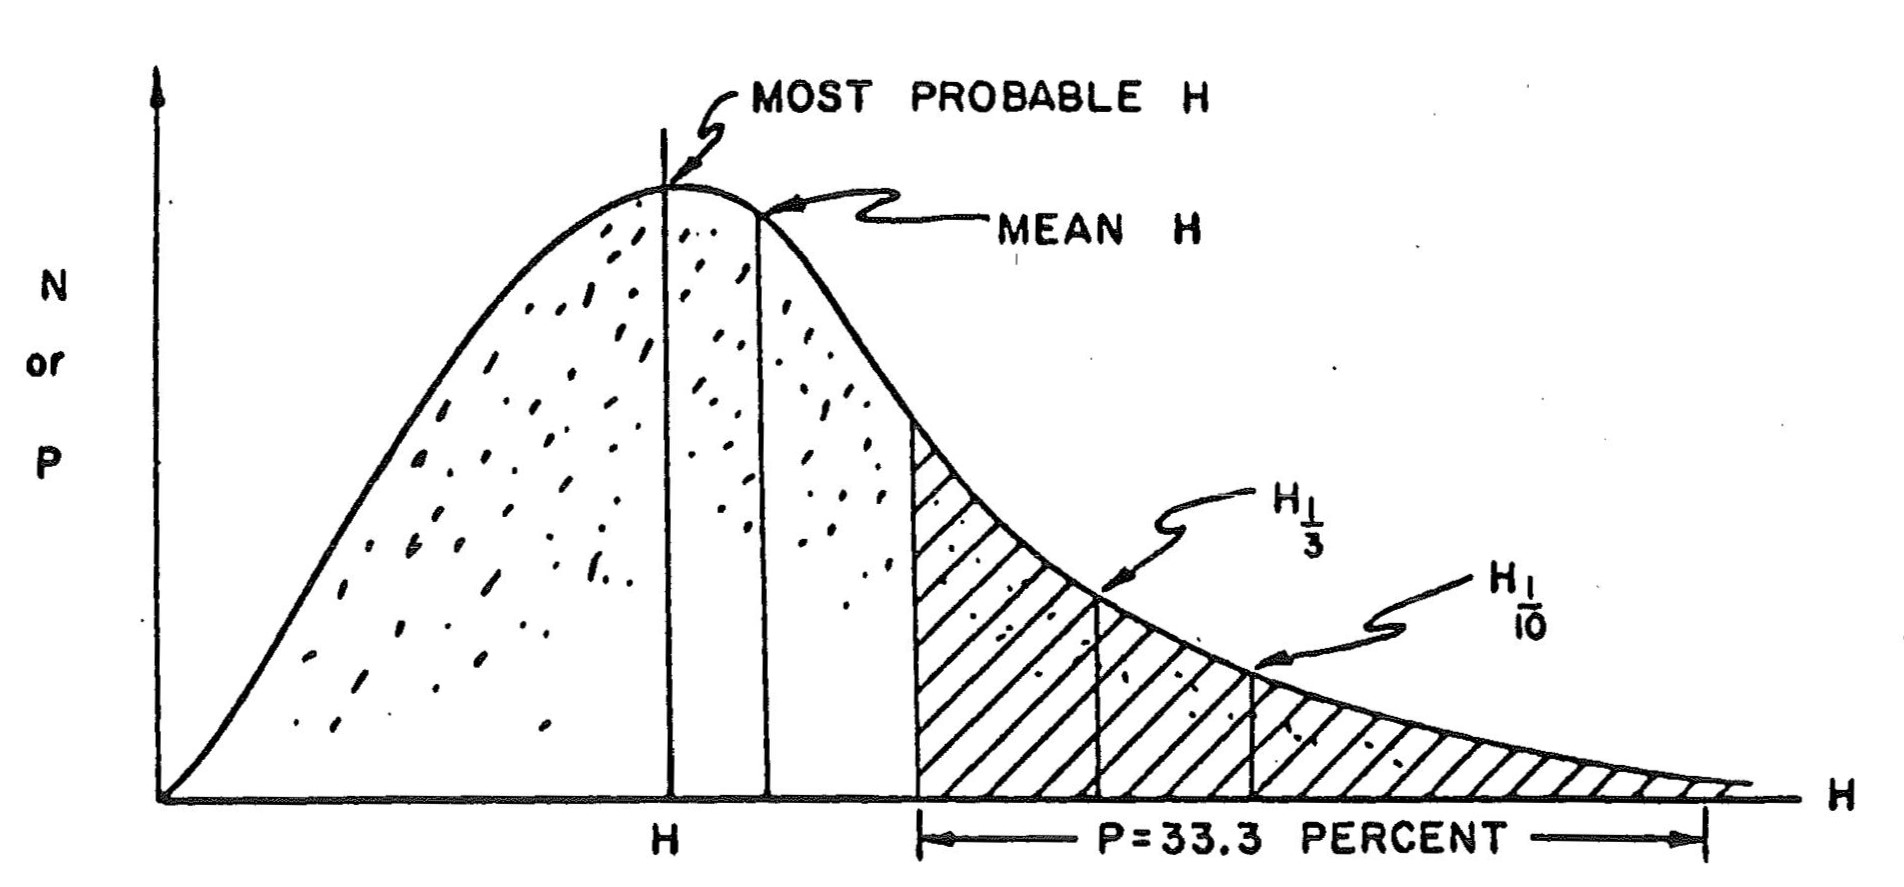
\includegraphics[width=.75\textwidth]{02_figures/Bretschneider_1965_wavedist.jpg}
        \caption{Statistical distribution of wave heights \bcitep{bretschneider.1965}}
        \label{fig:wavestats}
\end{figure}

\pagebreak

\subsubsection*{Wave Period}

Defined as the time interval between the start and the end of a wave. Some characteristics of wave period can be derived to define wave spectrum.

\subsubsection*{Wave Spectrum}

The most important form in which ocean waves are described. Wave spectrum characterises all possible observations of the waves which include wave heights, frequencies i.e. period and wave direction. For example, \bcitet{BitnerGregersen.2005} stated that the state of the sea can be described through the significant height $H_{1/3}$ and spectral peak period $\text{T}_p$ with the help of Torsethaugen peak, given the spectral peak period of fully developed sea $\text{T}_f$ and constant $a_f = 6.6$  \bcitep{K.Torsethaugen.2004}. 

\begin{equation}\label{eqn:T_p_spectralpeak}
    \text{T}_p = a_f\cdot H_{1/3}
\end{equation}
\begin{equation}
    \label{eqn:H_s_and_Tp}
    \text{Sea State (SS)} = 
    \begin{cases}
        \begin{aligned}
            &\text{Swell dominated}  &&\text{\textbf{if}} \quad \text{T}_p > \text{T}_f \\ 
            &\text{Wind sea dominated} && \text{\textbf{if}} \quad \text{T}_p \leqslant \text{T}_f 
        \end{aligned}     
    \end{cases} 
\end{equation}

\pagebreak

\section{General concept of ship propulsion}\label{sec:power_calc}

A ship's bunker fuel consumption in actual operating conditions is affected by several factors including the operating parameter of the ship's engine, propeller efficiency, and encountered resistance by the ship. Furthermore, a ship's propulsion power is correlated to the sailing speed (SOG) and meteorological conditions \bcitep{XiaoLang.2020}. Therefore, in addition to the calm water resistance $R_{CALM}$, the additional resistance caused by wind $R_{AA}$ and wave $R_{AW}$ should be considered to estimate the total resistance of the ship $R_{TOTAL}$. The power needed to propel a ship forward at a given ship STW $v_S$, to overcome $R_{TOTAL}$ is defined as \textbf{effective power $P_e$}:

\begin{equation}\label{eqn:R_tot}
    R_{TOTAL} = R_{CALM} + R_{AW} + R_{AA} 
\end{equation}

\begin{equation}\label{eqn:P_e}
    P_e = R_{TOTAL}\cdot v_{S}
\end{equation}

The effective power $P_e$ is transmitted through the shaft connected to the main engine of the ship which generates power to rotate the propeller of the ship, which is termed as \textbf{brake power of the engine, $P_b$}. The brake power can be calculated through effective power by considering the \textbf{shaft efficiency $\eta_s$, hull efficiency $\eta_h$, relative rotative efficiency $\eta_r$ and open water efficiency $\eta_o$}:

\begin{equation}\label{eqn:P_b}
    P_b = \frac{P_e}{\eta_s\cdot\eta_h\cdot\eta_r\cdot\eta_o}
\end{equation}

The bunker fuel consumption can then be calculated by multiplying the brake power $P_b$ with the Specific Fuel Oil Consumption (SFOC) and the operation time $\tau_{OP}$:

\begin{equation}\label{eqn:FOC}
    FOC = P_b\cdot SFOC\cdot \tau_{OP} 
\end{equation}

\subsection{Ship dimensions and form coefficients}\label{sec:Ship_design_param}

\subsubsection*{Principal Dimension of a vessel}

The summary of important ship dimensions and parameters are shown in \Cref{fig:biran14_shipside} and \Cref{fig:biran14_shipfront} \bcitep{Biran.2014}:

\begin{figure}[ht]
    \centering
    \begin{minipage}[b]{0.5\linewidth}
        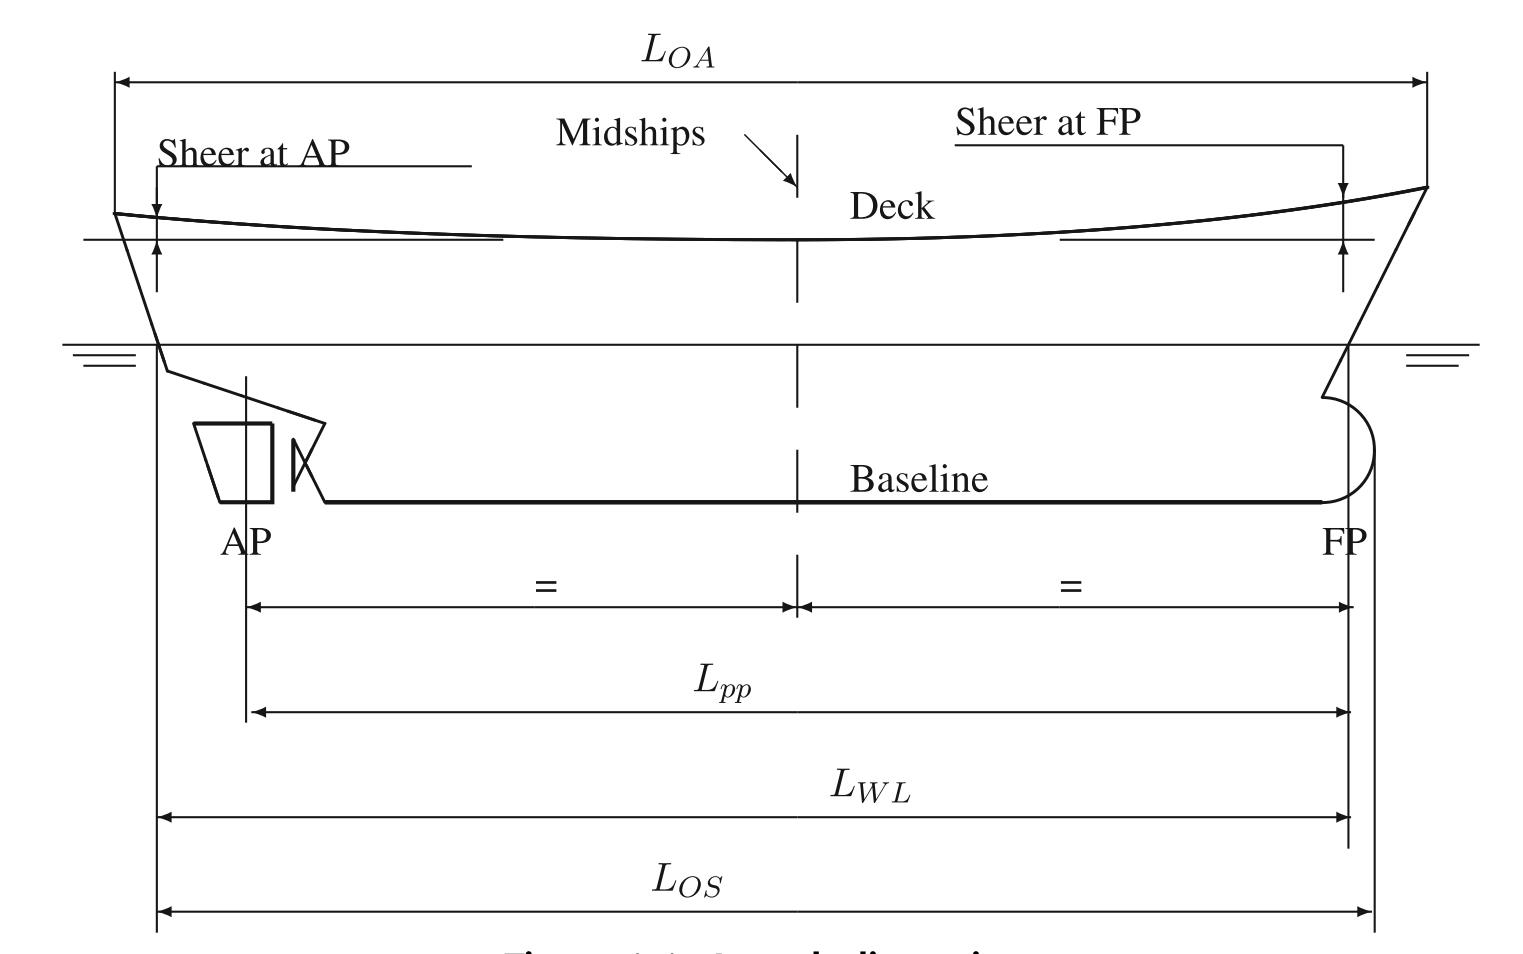
\includegraphics[width=\linewidth]{02_figures/biran14_shipside .jpg}
        \caption{Side view of a vessel}
        \label{fig:biran14_shipside}
    \end{minipage}
    \hfill
    \begin{minipage}[b]{0.45\linewidth}
        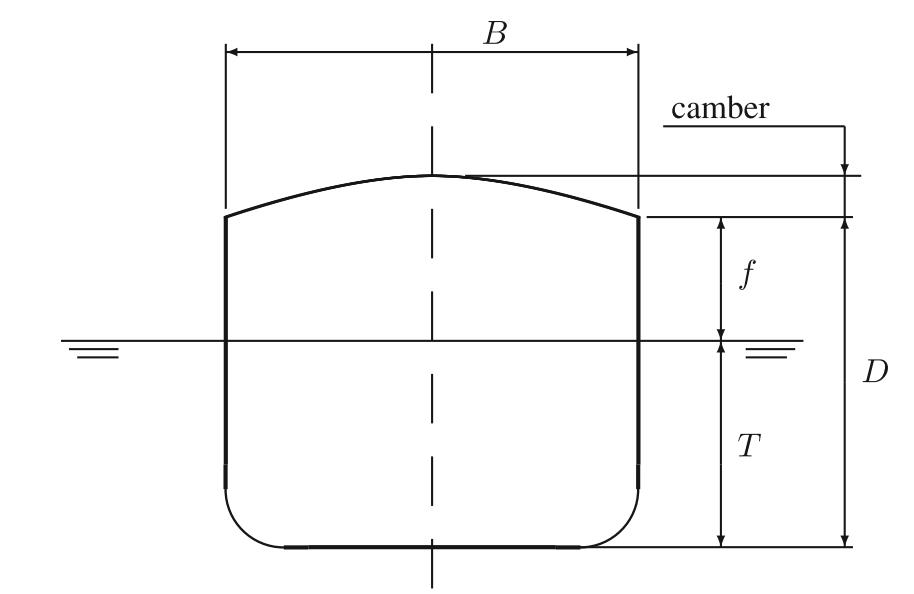
\includegraphics[width=\linewidth]{02_figures/biran14_frontship .jpg}
        \caption{Front view of a vessel}
        \label{fig:biran14_shipfront}
    \end{minipage}
\end{figure}

The outer surface of the ship is usually not uniform as not all plates have the same thickness, Therefore the hull surface is measured with respect to the inner surface of the plating which is termed as \emph{moulded surface} of the hull. All dimensions measured to this surface are defined as \emph{moulded} dimensions whereas dimensions measured to the outer surface of the hull or of an appendage are qualified as \emph{extreme} dimensions \bcitep{Biran.2014}.

\subsubsection*{Coefficients of form}

The form coefficients are non-dimensional numbers required to classify the hulls and to find relationships between forms and their properties, the summary of some important form coefficients are summarised in \Cref{fig:man_formcoeff} 

\begin{figure}[ht]
    \centering
        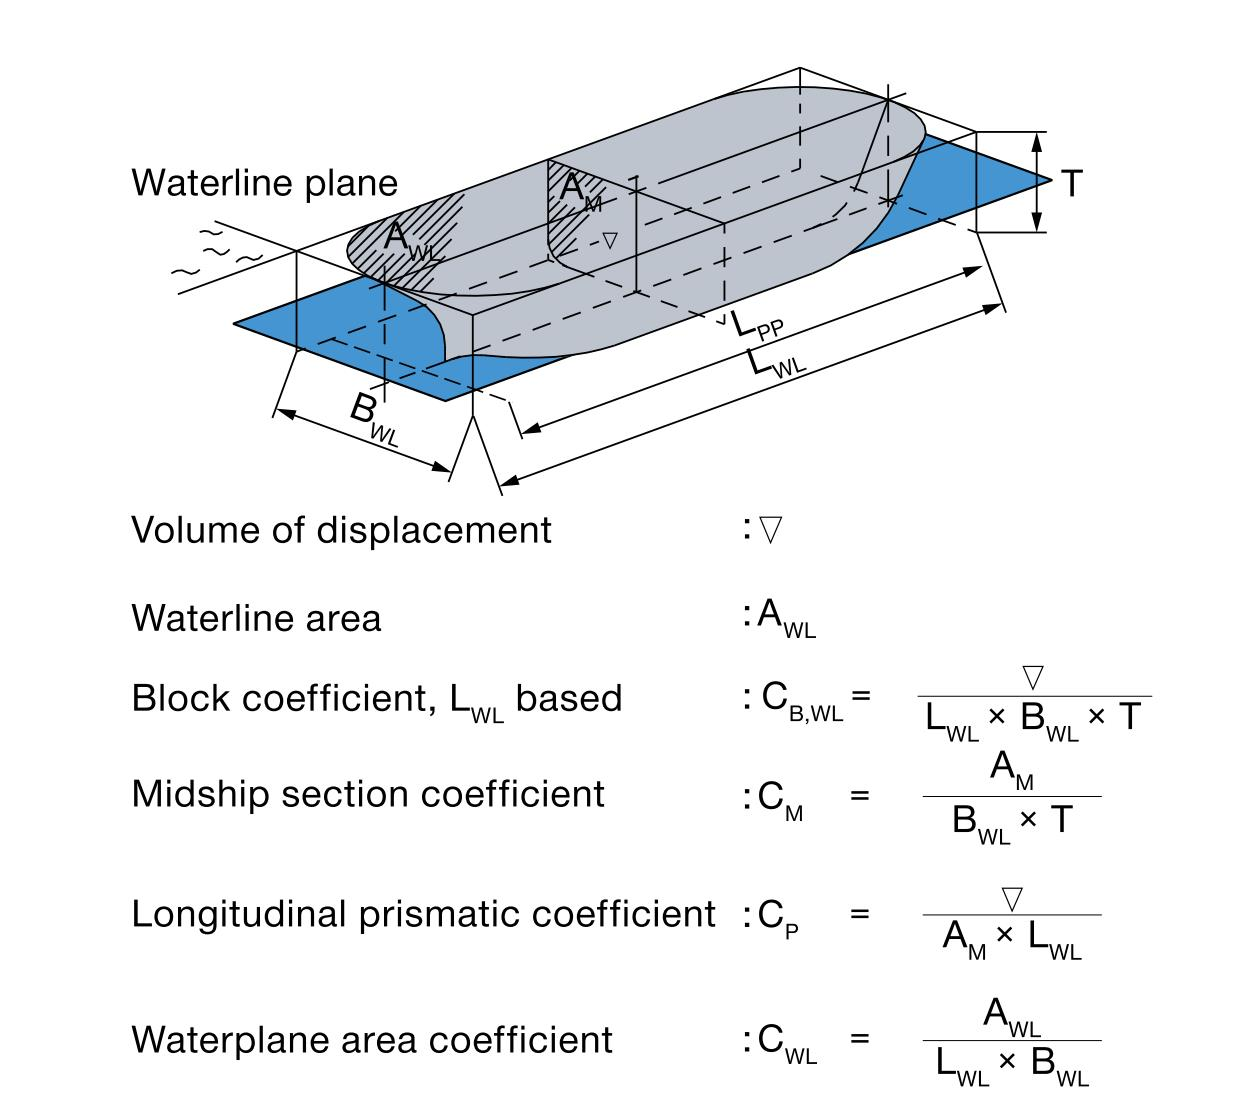
\includegraphics[width=.6\textwidth]{02_figures/man11_shipcoeff.jpg}
        \caption{Form coefficients \bcitep{Diesel.2011}}
        \label{fig:man_formcoeff}
\end{figure}

\subsubsection*{Block Coefficient}
\textbf{Block Coefficient $C_B$} is defined as the ratio of moulded displacement volume to the volume of parallelepiped (rectangular block) with dimensions $L,B$ and $T$. Alternatively, \bcitet{Schneekluth.1998} provided an estimation of the value using the Froude number within the range of $0.15 < Fr < 0.32$

\begin{equation}
    \label{eqn:Cb_Schneekluth}
    C_b = -4.22 + 27.8\sqrt{Fr} - 39.1Fr + 46.6Fr^3
\end{equation}

The Froude number $Fr$ is defined with the following equation:

\begin{equation}
    \label{eqn:Froude_Number}
    Fr = \frac{v}{\sqrt{gL_{WL}}}
\end{equation}

\subsubsection*{Midship Coefficient}
\textbf{Midship Coefficient $C_M$} is defined as the ratio of the midship-section area $A_M$ to the product of breadth and draught, $BT$. According to \bcitet{Schneekluth.1998}, changing $C_M$ value will have an effect on separation resistance and wave resistance. \bcitet{jensen1994moderne} presented a method based on regression equation on a graph to calculate $C_M$:  

\begin{equation}
    \label{eqn:CM_jensen}
    C_M = \frac{1}{1+(1-C_B)^{3.5}}
\end{equation}

\begin{figure}[ht]
    \centering
        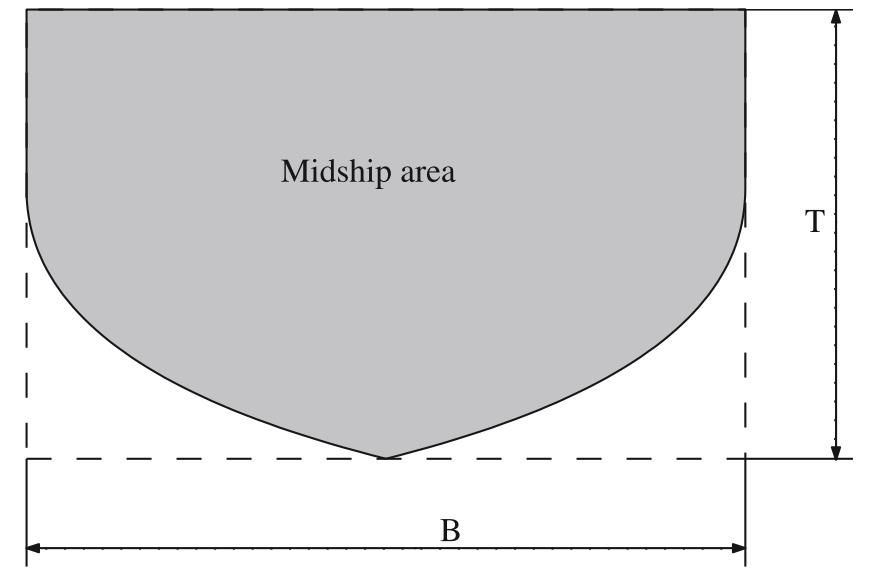
\includegraphics[width=.4\textwidth]{02_figures/biran14_cm.jpg}
        \caption{Definition of $C_M$ \bcitep{Biran.2014}}
        \label{fig:biran_cm}
\end{figure}

\subsubsection*{Prismatic Coefficient}

\textbf{Prismatic Coefficient $C_P$} is defined as the ratio of moulded displacement volume\footnote{In some notations it is denoted as $\nabla$} $V$. It is an indicator on how much of a cylinder with constant section $A_M$ and length $L$ is filled with submerged hull as shown in \Cref{fig:biran_cp}.

\begin{equation}
    \label{eqn:cp_ratio}
    C_P = \frac{C_B}{C_M}
\end{equation}

\begin{figure}[ht]
    \centering
        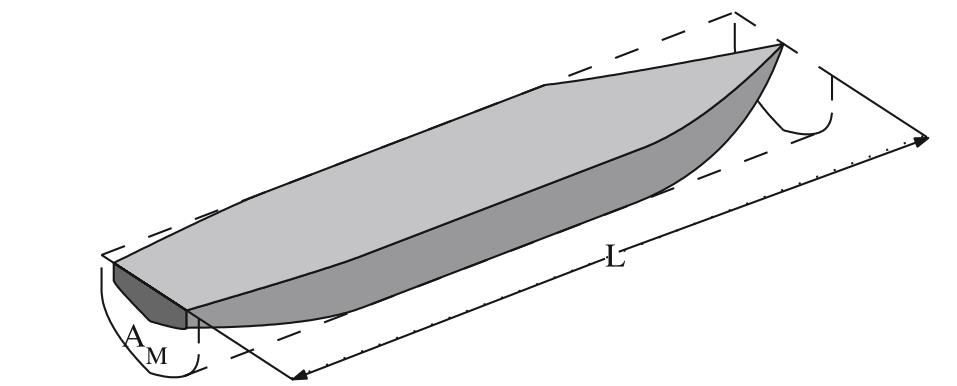
\includegraphics[width=.5\textwidth]{02_figures/biran14_cp.jpg}
        \caption{Definition of $C_P$ \bcitep{Biran.2014}}
        \label{fig:biran_cp}
\end{figure}

\pagebreak

\subsubsection*{Waterplane area coefficient}

\textbf{Waterplane area coefficient $C_{WP}$} is defined as the ratio between the ship's waterline area $A_{W}$ and the product of $L$ and $B$. In ship design, $C_{WP}$ significantly impacts resistance and stability \bcitep{Schneekluth.1998}. \bcitet{Diesel.2011} approximated that $C_{WP}$ is 0.10 higher than $C_B$, alternatively \bcitet{Schneekluth.1998} provided the following formulation for $C_{WP}$:

\begin{equation}
    \label{eqn:cwp_Schneekluth}
    C_{WP} = \frac{1+2C_B}{3}
\end{equation}

\begin{figure}[ht]
    \centering
        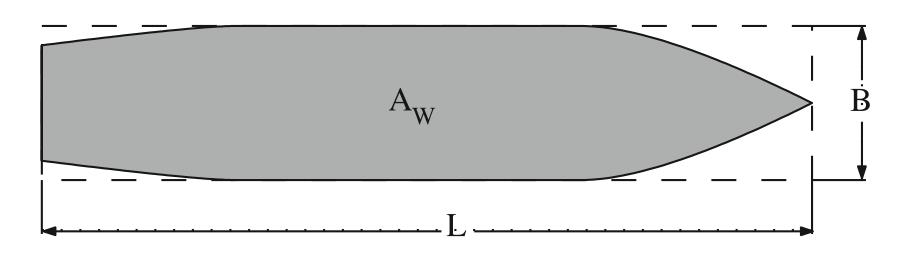
\includegraphics[width=.5\textwidth]{02_figures/biran14_cwp.jpg}
        \caption{Definition of $C_{WP}$ \bcitep{Biran.2014}}
        \label{fig:biran_cwp}
\end{figure}

\subsection{Holtrop \& Mennen's Method}\label{sec:holtrop_mennen_calc}

This power prediction method was applied in the late 1970s and early 1980s by J. Holtrop and G.G.J Mennen and it was based on regression analysis of vast model tests and trial data of MARIN, the model basin in Wageningen, The Netherlands. This gives Holtrop-Mennen method a wide applicability range and the only method that adopted the use of the ITTC form factor $k$. The resistances in this method are calculated as dimensional force. Furthermore, the method also gives estimates of hull-propeller interaction, thrust deduction, full-scale wake fraction and relative rotative efficiency \bcitep{Birk.2019}. 

\begin{table}[ht]
    \footnotesize
    \centering
    % \resizebox {\textwidth}{!}
    {\begin{tabular}{ p{0.45\linewidth} p{0.08\linewidth} p{0.38\linewidth}  }
    \hline
    \textbf{Parameter} & \textbf{Symbol} & \textbf{Remarks} \\
    \hline
    Required Parameters&&\\
    \hline
    Length in waterline & $L_{WL}$\\
    Moulded breadth & $B$ \\
    Moulded mean draught & $T$ & typically $T = \frac{1}{2}(T_A+T_F)$ \\
    Moulded draught at aft perpendicular & $T_A$ & \\ 
    Moulded draught at forward perpendicular & $T_F$\\
    Volumetric displacement (molded) & $V$ & alternatively use the block \mbox{coefficient} as $C_B = V/BTL_{WL}$\\
    Prismatic coefficient (based on $L_{WL}$) & $C_P$ \\
    Midship section coefficient & $C_M$ & or use $C_M=C_B/C_P$ \\
    Waterplane area coefficient & $C_{WP}$ & may have to be estimated in early design stages\\
    Longitudinal Centre of buoyancy & $\ell_{CB}$ &positive forward; with respect to $L_{WL}/2$ in percent of $L_{WL}$\\
    Area of ship and cargo above waterline & $A_V$ & projected in direction of $v_S$\\
    Immersed transom area & $A_T$ & measured at rest\\
    Transverse area of bulbous bow & $A_{BT}$ & Measured at forward perpendicular \\
    Height of centre $A_{BT}$ above basis & $h_B$ & has to be smaller than $0.6T_F$ \\
    Propeller Diameter & $D$ \\
    Propeller expanded area ratio & $A_E/A_0$ \\
    Stern shape parameter & $C_{stern}$ \\
    \hline
    Optional Parameters&&\\
    \hline
    Wetted surface (hull) & $S$\\
    Wetted Surface of appendages & $S_{App}$ & bilge keels, stabiliser fins, etc.\\
    Half angle of waterline entrance & $i_E$ \\
    Diameter of bow thruster tunnel & $d_{TH}$ \\
    \hline
    \end{tabular}}
\caption{Required and optional input parameters for Holtrop \& Mennen's method according to \bcitet{Birk.2019}}
\label{tbl:holtrop_params}
\end{table}

\subsubsection*{Application Range}

The publication from \bcitet{Holtrop.1978,Holtrop.1982,Holtrop.1984} does not provide explicit information regarding the application range of the method. However, from the experience of \bcitet{Birk.2019}, reasonable estimates from the method can be achieved for the following conditions: \\

\begin{equation}
    \label{eqn:holtrop_cond}
    % \begin{multlined}
    \begin{gathered}
        Fr \leqslant 0.45 \\
        0.55 \leqslant C_p \leqslant 0.85 \\
        3.9 \leqslant \frac{L}{B} \leqslant 9.5
    \end{gathered}
    % \end{multlined}
\end{equation}

\subsubsection{Calm water resistance}\label{sec:Calm_Resistance}

The calm water resistance $R_{CALM}$ is broken down into several components and can be approximated using the following relation:

\begin{equation}\label{eqn:R_calm}
    R_{CALM} = R_F(1+k_1) + R_{APP} + R_W + R_B + R_{TR} + R_A
\end{equation}

\subsubsection*{Frictional Resistance $R_F$}

\textbf{$R_F$} is calculated using the ITTC-1957 frictional resistance correlation line $C_F$ as the basis of a representation of a resistance plate with a wetted surface area $S$ of bare hull. 

\begin{equation}\label{eqn:R_f}
    R_F = \frac{1}{2}\rho v_{S}^2 S C_F 
\end{equation}

The frictional coefficient $C_F$ can be calculated through the Reynold number $Re$ for a given ship speed $v_{S}$ and kinematic viscosity $\nu$:

\begin{equation}\label{eqn:C_F}
    C_F = \frac{0.075}{[\log_{10}(Re)-2]^2} \quad \textbf{where} \quad Re = \frac{v_{S}L_{WL}}{\nu}
\end{equation}

If not known, then the wetted surface area of bare hull $S$ can be estimated by the following formula:

\begin{equation}\label{eqn:S_bh}
    S = c_{23}L_{WL}(2T+B)\sqrt{C_M}+2.38\frac{A_{BT}}{C_B}
\end{equation}

with the factor $c_{23}$ given as :

\begin{equation}\label{eqn:c_23}
    c_{23} = \biggl[0.453 + 0.4425C_B - 0.2862C_M - 0.003467\frac{B}{T} + 0.3696C_{WP} \biggr]
\end{equation}

The flat plate resistance is subsequently adjusted by including a form factor $k$ during the calculation of total resistance. The constant $c_{14}$ must be determined first to calculate form factor $k$, which serves the purpose of capturing the impact of the aft body shape.   

\begin{equation}\label{eqn:c_14}
    c_{14} = 1.0 + 0.011C_{stern} \quad \textbf{with} \quad \begin{array}{l c}
        \text{Aft body shape} & C_{stern}\\
        \hline
        \text{Pram with gondola} & -25 \\
        \text{V-shaped sections} & -10 \\
        \text{Normal sections} & 0 \\
        \text{U-shaped sections} & +10 \\
        \hline
    \end{array}
\end{equation}

To complete the required input for the calculation of $(1+k_1)$, the length of run $L_R$ can be estimated from the following equation:

\begin{equation}\label{eqn:L_R}
    L_R = L_{WL}(\frac{1-C_P+0.06C_P\ell_{CB}}{4C_P-1})
\end{equation}

The formula by \bcitet{Guldhammer.1974} can be used if $\ell_{CB}$ is not known:

\begin{equation}
    \label{eqn:lcb}
    \ell_{CB} = -(0.44Fr - 0.094)
\end{equation}

Then, the form factor $(1+k_1)$ can be determined with the constant $c_{14}$, the length of run $L_R$ and input values from \Cref{tbl:holtrop_params}.

\begin{multline}\label{eqn:1+k1}
    1+k_1 = 0.93 + 0.487118c_{14}\Biggl[ \Biggl(\frac{B}{L_{WL}}\Biggr)^{1.06806}  \Biggl(\frac{T}{L_{WL}}\Biggr)^{0.46106} \\ 
    \Biggl(\frac{L_{WL}}{L_R}\Biggr)^{0.121563} \Biggl(\frac{L_{WL}}{V}\Biggr)^{0.36486} (1-C_p)^{-0.604247} \Biggr] 
\end{multline}

\subsubsection*{Appendage Resistance}

An appendage is defined as the addition(s) to the main part or main structure of a vessel \bcitep{Molland.2011}. Examples of appendages include rudders, shaft brackets, skeg and bilge keels. The form factors associated with these appendages, denoted as $k_{2_i}$ are presented in \Cref{tbl:k2i_values}. In practice, reasonable estimates can be made based on these form factors, as model tests are not the most suitable method for accurately quantifying appendage resistance. Furthermore, the effects of appendages are typically considered as a whole and not as individual units \bcitep{Birk.2019}.\\

\begin{table}[ht]
    \footnotesize
    \centering
    {\begin{tabular}{ p{0.6\linewidth} c}
    \hline
    Appendage & $k_{2_i}$ value \\
    \hline
    rudder behind skeg & $0.2-0.5$ \\
    rudder behind stern & $0.5$ \\
    twin screw rudder (slender) & $1.5$ \\
    twin screw rudder (thick) & $2.5$ \\
    shaft brackets & $2.0-4.0$ \\
    skeg & $0.5-1.0$ \\
    strut bossing & $2.0-3.0$ \\
    hull bossing & $1.0$ \\
    exposed shafts (angle with buttocks about 10 degrees) & $1.0$ \\
    exposed shafts (angle with buttocks about 20 degrees) & $4.0$ \\
    stabiliser fins & $1.8$ \\
    dome & $1.7$ \\
    bilge keels & $0.4$ \\ 
    \hline
    \end{tabular}}
\caption{Approximate values for appendage form factors $k_{2_i}$}\label{tbl:k2i_values}
\end{table}

The equivalent form factor for multiple appendages, $(1+k_{2_i})_{eq}$ is given by:

\begin{equation}\label{eqn:k2eq}
    (1+k_{2_i})_{eq} = \frac{\sum_i(1+k_{2_i})S_{APP_i}}{\sum_iS_{APP_i}}
\end{equation}

If bow thruster is present, the resistance due to the bow thruster tunnel $R_{TH}$ can be obtained through:

\begin{equation}\label{eqn:R_th}
    R_{TH} = \rho v_S^2 \pi d_{TH}^2 C_{D_{TH}} \quad \textbf{where} \quad C_{D_{TH}} = 0.003 + 0.003 \Biggl( \frac{10{d_{TH}}}{t} - 1 \Biggr) 
\end{equation}

The coefficient $C_{D_{TH}}$ defines the drag coefficient for the tunnel, and it ranges between $0.003$ and $0.012$. Smaller values indicate thrusters which are in the cylindrical part of the bulbous bow. The coefficient can also be estimated using the equation by \bcitet{Hollenbach.1999} in \Cref{eqn:R_th}.\\

With that, the appendage resistance $R_{APP}$ can be calculated using:

\begin{equation}\label{eqn:R_app}
    R_{APP} = \frac{1}{2}\rho v_S^2 (1+k_{2_i})_{eq} C_F \sum_i S_{APP_i} + \sum R_{TH}
\end{equation}

\subsubsection*{Wave Resistance}

The estimation of wave resistance $R_W$ is dependent on Froude number $Fr$, and it is subdivided into three categories.\footnote{Considering the length of the equations, only the scenario where $Fr \leqslant 0.4$ will be thoroughly examined in this thesis. The formulations of $R_W$ for other ranges of Froude number can be referenced in the studies by \bcitet{Holtrop.1984} and \bcitet{Birk.2019}}:

\begin{equation}
    \label{eqn:case_Rw}
    R_W(Fr) = 
    \begin{cases}
        \begin{aligned}
        &R_{W_a}(Fr) && \textbf{if} \quad Fr \leqslant 0.4 \\
        &\text{Interpolation} && \textbf{if} \quad 0.4 < Fr \leqslant 0.55 \\
        &R_{W_b}(Fr) && \textbf{if} \quad Fr > 0.5 \\
    \end{aligned}
    \end{cases}
\end{equation}

The wave resistance for $R_{W_a}(Fr)$ can be calculated using:

\begin{equation}\label{eqn:R_w_low}
    R_{W_a}(Fr) = c_1 c_2 c_5 \rho g V  \exp \biggl[ m_1 Fr^d + m_4 \cos(\lambda Fr ^{-2}) \biggr]
\end{equation}

And consequently for $R_{W_b}(Fr)$:

\begin{equation}\label{eqn:R_w_high}
    R_{W_b}(Fr) = c_{17} c_2 c_5 \rho g V  \exp \biggl[ m_3 Fr^d + m_4 \cos(\lambda Fr ^{-2}) \biggr]
\end{equation}

The Froude number range remaining between $0.4 < Fr \leqslant 0.55$ is determined using interpolation between equations \Cref{eqn:R_w_low} and \Cref{eqn:R_w_high}. It is important to note that this specific range of Froude numbers (0.4 to 0.55) is generally considered uneconomical for ship operation, and ships do not typically operate within this speed range for extended periods \bcitep{Birk.2019}.

\begin{equation}\label{eqn:R_w_mid}
    R_W(Fr) = R_{W_a}(0.4) + \frac{20Fr-0.8}{3} \biggl[ R_{W_b}(0.55) - R_{W_a}(0.4)\biggr]
\end{equation}

To compute each of the constants in \Cref{eqn:R_w_low}, The following equations are presented, note that the calculations for the \textbf{$\cos (\lambda Fr^{-2})$} are in \textbf{Radians}:

\begin{equation}\label{eqn:c_7}
    c_7 = \begin{cases}
        \begin{aligned}
        &0.229577\biggl(\frac{B}{L_{WL}} \biggr)^\frac{1}{3}  &&\textbf{if} \quad \frac{B}{L_{WL}} \leqslant 0.11 \\
        &\frac{B}{L_{WL}}  &&\textbf{if}  \quad 0.11 < B/L_{WL} \leqslant 0.25\\
        &0.5 - 0.0625\frac{L_{WL}}{B}  &&\textbf{if}  \quad B/L_{WL}>0.25 
        \end{aligned} 
    \end{cases}
\end{equation}

\begin{equation}\label{eqn:c_1}
    c_1 = 2223105c_7^{3.78613}\biggl( \frac{T}{B}\biggr)^{1.07961}(90-i_e)^{1.37565}
\end{equation}

$i_E$ is defined as the half angle of the waterline entrance and the estimation can be calculated by:

\begin{equation}\label{eqn:i_e}
    i_E = 1+89 e^{a}
\end{equation}

and $a$ can be obtained through:

\begin{multline}\label{eqn:a_const_ie}
    a = -\biggl[ \biggl(\frac{L_{WL}}{B}\biggr)^{0.80856} \biggl(1 - C_{WP}\biggr)^{0.30484} \biggl[1 - C_P - 0.0225\ell_{CB}\biggr]^{0.6367} \\
    \biggl(\frac{L_R}{B}\biggr)^{0.34574} \biggl(\frac{100V}{L_{WL}^3}\biggr)^{0.16302} \biggr]
\end{multline}

\begin{equation}\label{eqn:c3}
    c_3 = 0.56 \frac{A_{BT}}{\left[BT\left(0.31 \sqrt{A_{BT}} + T_F + h_B\right)\right]}
\end{equation}

\begin{equation}\label{eqn:c2}
    c_2 = e^{(-1.89\sqrt{c_3})}
\end{equation}

\begin{equation}
    \label{eqn:c15}
    c_{15} =
    \begin{cases}
        \begin{aligned}
            & -1.69385 && \textbf{if} \quad \frac{L_{WL}^2}{V} \leqslant 512 \\
            & -1.69385 + \frac{\frac{L_{WL}}{V^{(1/3)}}-8}{2.36}&& \textbf{if} \quad 512 < \frac{L_{WL}^2}{V} \leqslant 1726.91 \\
            & 0 && \textbf{if} \quad \frac{L_{WL}^2}{V} > 1726.91
        \end{aligned}
    \end{cases}
\end{equation}

\begin{equation}
    \label{eqn:c16}
    c_{16} = 
    \begin{cases}
        \begin{aligned}
            & 8.07981C_P - 13.8673C_P^2 + 6.984338C_P^3 && \textbf{if} \quad C_P \leqslant 0.8 \\
            & 1.73014 - 0.7067C_P && \textbf{if} \quad C_P > 0.8
        \end{aligned}
    \end{cases}
\end{equation}

\begin{equation}
    \label{eqn:d}
    d = -0.9
\end{equation}

\begin{equation}
    \label{eqn:lambda}
    \lambda = 
    \begin{cases}
        \begin{aligned}
            &1.446C_P - 0.03\frac{L_{WL}}{B} && \textbf{if} \quad \frac{L_{WL}}{B} \leqslant 12 \\
            &1.446C_P - 0.36 && \textbf{if} \quad \frac{L_{WL}}{B} > 12 \\
        \end{aligned}
    \end{cases}
\end{equation}

\begin{equation}
    \label{eqn:m1}
    m_1 = 0.0140407C_P - 0.03\frac{L_{WL}}{B} - 1.75254\frac{V^{(1/3)}}{L_{WL}} - 4.79323\frac{B}{L_{WL}} - c{16}
\end{equation}

\begin{equation}
    \label{eqn:m4}
    m_4 = 0.4 c_{15} \exp{(-0.034Fr^{-3.29})}
\end{equation}

\subsubsection*{Resistance of bulbous bow}

The approximation of the resistance due to bulbous bow $R_B$ can be obtained through the immersion Froude number $F_{r_i}$ for the bulbous bow and the constant $P_B$ which is a measure of the emergence of the bow: 

\begin{equation}
    \label{Fr_immersion}
    Fr_i = \frac{v_S}{\sqrt{g(T_F-h_b-0.25 \sqrt{A_{BT}})+0.15v_S^2}}
\end{equation}

\begin{equation}
    \label{Pb}
    P_B = 0.56 \frac{\sqrt{A_{BT}}}{T_F-1.5h_B+h_F}
\end{equation}

\begin{equation}
    \label{eqn:Rbulb}
    R_B = 0.11 \rho g (\sqrt{A_{BT}})^3 \frac{Fr_{i}^3}{1+Fr_{i}^2}e^{(-3.0P_B^-2)}
\end{equation}

\begin{figure}[ht]
    \centering
    \begin{minipage}[b]{0.45\linewidth}
        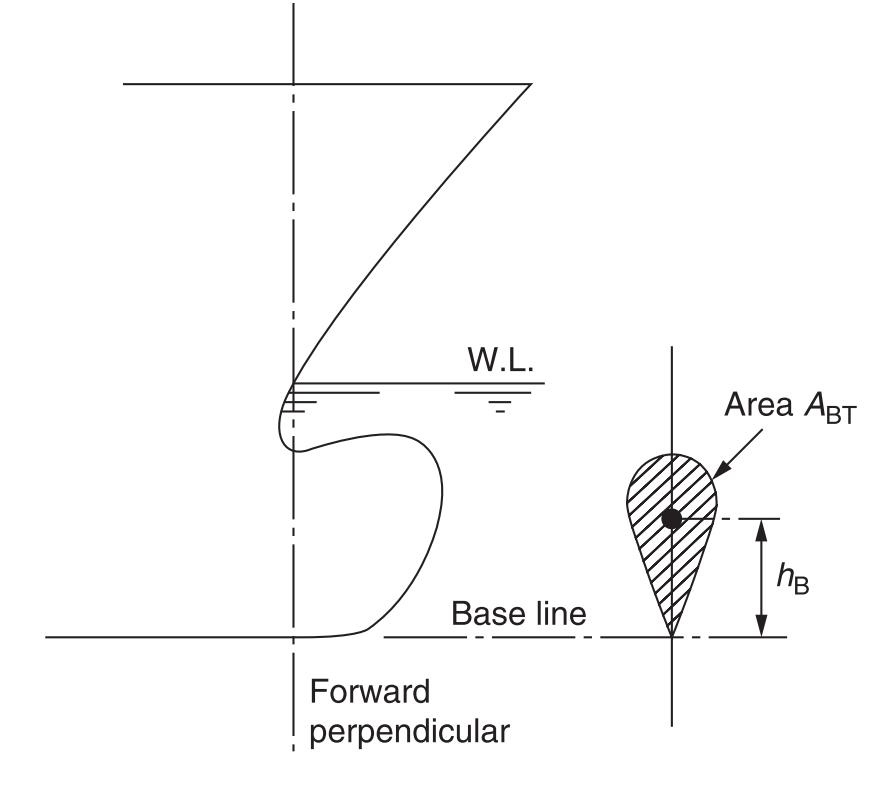
\includegraphics[width=\linewidth]{02_figures/Molland11_bulb.jpg}
        \caption{Bulbous bow definition \bcitep{Molland.2011}}
        \label{fig:molland11_bow}
    \end{minipage}
    \hfill
    \begin{minipage}[b]{0.45\linewidth}
        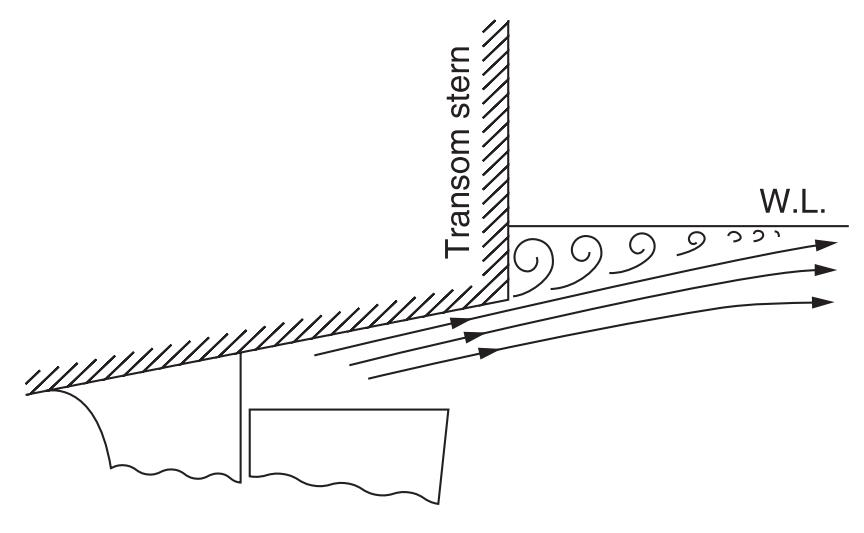
\includegraphics[width=\linewidth]{02_figures/molland11_transom.jpg}
        \caption{Flow around immersed transom stern \bcitep{Molland.2011}}
        \label{fig:molland1_transom}
    \end{minipage}
\end{figure}

\subsubsection*{(Immersed) Transom Resistance}

The term transom refers to the flat section located at the stern of the ship. When the transom becomes immersed in water, it leads to pressure loss, resulting in resistance. This resistance is denoted by the term $R_{TR}$ and is associated with an immersed transom area $A_T > 0$. The transom resistance can be described as a function of the depth Froude number $Fr_{T}$:

\begin{equation}
    \label{eqn:Fr_t}
    Fr_T = \frac{v_S}{\sqrt{\frac{2gA_T}{(B+BC_{WP})}}}
\end{equation}

The expression $A_T/(B+BC_{WP})$ is a measure for the average draught of the transom. When the average draught is smaller than the speed, there will be clean separation of the flow at transom edge and the resistance due to transom vanishes. Immersion resistance $R_{TR}$ is considered if $Fr_{T} > 5$ 

\begin{equation}
    \label{eqn:c6}
        c_6 = 
        \begin{cases}
            \begin{aligned}
              &0.2(1-0.2Fr_T) && \textbf{if} \quad Fr_T < 5 \\
              & 0 && \textbf{if} \quad Fr_T > 5  
            \end{aligned}
        \end{cases}
\end{equation}

\begin{equation}
    \label{eqn:R_transom}
    R_{TR} = \frac{1}{2}\rho v_S^2 A_T c_6
\end{equation}

\subsubsection*{Correlation allowance resistance}

The resistance term $R_A$ considers other effects that are not captured by other resistance components. 

\begin{equation}
    \label{eqn:c4}
    c_4 =
    \begin{cases}
        \begin{aligned}
            &\frac{T_F}{L_{WL}} && \textbf{if} \quad \frac{T_F}{L_{WL}} \leqslant 0.04 \\
            &0.04 && \textbf{if} \quad \frac{T_F}{L_{WL}} >0.04 
        \end{aligned}
    \end{cases}
\end{equation}

\pagebreak

The correlation allowance coefficient $C_A$ and subsequent correlation resistance is defined as:

\begin{equation}
    \label{eqn:Ca_correlation}
    C_A = 0.00546(L_{WL}+100)^{-0.16} - 0.00205 + 0.003\frac{L_{WL}}{7.5}C_{B}^4c_2(0.04-c_4)
\end{equation}

\begin{equation}
    \label{eqn:R_a}
    R_A = \frac{1}{2}\rho v_S^2 C_A (S+\sum S_{APP})
\end{equation}

\subsubsection{Added resistance due to wind}\label{sec:wind_resistance}

The magnitude of added resistance caused by wind, $R_{AA}$, is determined by the area of the ship superstructure and relative wind. Therefore, for a ship with large lateral areas above the water level, this added resistance due to wind can be significant. The estimation of added resistance due to wind in this thesis consider the method by \bcitet{Blendermann.1994}:

\begin{equation}
    \label{eqn:Raa_blendermann}
    R_{AA} = \frac{\rho_{air}}{2}u^2A_{L}CD_l \frac{\cos{(\varepsilon)}}{1-\frac{\delta}{2}(1-\frac{CD_l}{CD_t}\sin^2{(2\varepsilon)})}
\end{equation}

Where $u$ is the apparent wind velocity, $A_L$, the lateral plane area, $\varepsilon$, the apparent wind angle ($\varepsilon = 0$ in headwind), $\delta$ the cross-force parameter, and coefficients $CD_t$ and $CD_l$ the non-dimensional drag in beam wind and headwind. For given true wind velocity $u_{TW}$ and true wind angle (TWA), $\beta$, The calculation for the apparent wind $u$ and apparent wind angle $\epsilon$ is performed using the following equations:

\begin{equation}
    \label{eqn:u_AW}
    u = \sqrt{u_{\text{TW}}^2 + v_S^2 + 2 \cdot u_{\text{TW}} \cdot v_S \cdot \cos(\beta)}
\end{equation}

\begin{equation}
    \label{eqn:epsilon_AWA}
    \frac{u_{TW}}{\sin(\varepsilon)} = \frac{u}{\sin({\beta})}
\end{equation}

\begin{figure}
    \centering
        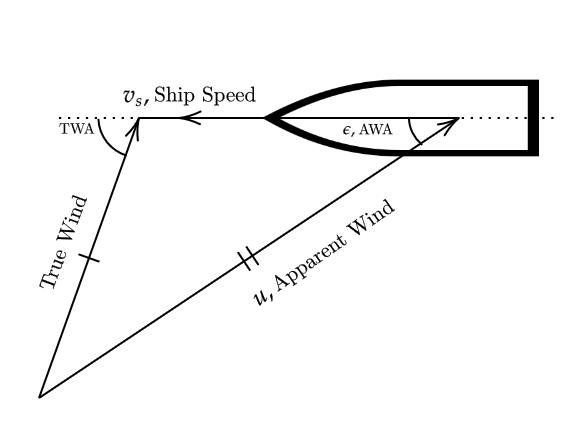
\includegraphics[width=.6\textwidth]{02_figures/AWA_TWAc.png}
        \caption{Apparent and true wind \bcitep{Knudsen.2013}}
        \label{fig:AWA_TWA}
\end{figure}

According to \bcitet{Schneekluth.1998}, maximum wind resistance is encountered when $0^\circ<\varepsilon<20^\circ$ and it is more convenient to express the longitudinal drag with respect to the frontal area $A_F$. Typical values for the constants are summarised in \Cref{tbl:BlendermannCoeff}

\begin{equation}
    \label{eqn:CDlaf}
    CD_{lAF} = CD_l \frac{A_L}{A_F}
\end{equation}

\begin{table}[ht]
    \footnotesize
    \centering
    % \resizebox {\textwidth}{!}
    {\begin{tabular}{ p{0.4\linewidth} c c c }
    \hline
    &\textbf{$CD_t$} & \textbf{$CD_{lAF}$} & \textbf{$\delta$} \\
    \hline
    Car carrier & 0.95 & 0.55 & 0.8 \\
    Cargo ship, container on deck, bridge aft & 0.85 & 0.65/0.55 & 0.40 \\
    Containership, loaded & 0.90 & 0.55 & 0.40 \\
    Ferry & 0.90 & 0.45 & 0.80\\
    LNG Tanker & 0.70 & 0.60 & 0.50 \\
    Passenger liner & 0.90 & 0.40 & 0.80 \\
    Speed boat & 0.90 & 0.55 & 0.60 \\
    Tanker, loaded & 0.70 & 0.90 & 0.40 \\
    Tanker, in ballast & 0.70 & 0.75 & 0.40 \\
    \hline        
    \end{tabular}}
\caption{Coefficients to estimate wind resistance}\label{tbl:BlendermannCoeff}
\end{table}

\pagebreak

\subsubsection{Added resistance due to wave}\label{sec:wave_resistance}

The added resistance due to wave, $R_{AW}$ is estimated using the STAWAVE-1 method recommended by \bcitet{ITTCProcedures.2014}. This method only considers waves encountered within the bow sector i.e. within $\pm 45^\circ$ off the bow and does not consider wave correction for other encounters. Also, STAWAVE-1 is valid for the following condition:

\begin{equation}
    \label{eqn:stawave_cond1}
    \text {Significant wave height:} \quad H_{1/3} = 2.25\leqslant\sqrt{L_{PP}/100} 
\end{equation}

\begin{equation}
    \label{eqn:stawave1}
    R_{AWL} = \frac{1}{16}\rho g H_{1/3}^2 B \sqrt{\frac{B}{L_{BWL}}} 
\end{equation}

In which, $L_{BWL}$ is the length of the bow on the water line to $95\%$ of maximum breadth.

\subsubsection{Efficiencies affecting brake power}\label{sec:Pb_efficiency}

\subsubsection*{Open water efficiency}

The open water efficiency \begin{math}\eta_O\end{math}, can be understood as the propeller working in open water conditions i.e. the propeller operates in a homogenous wake field with no hull in front of it. The curve of different propulsion devices with their respective efficiencies is summarised in the work of \bcitet{Breslin.1994}:

\begin{figure}[ht]
    \centering
        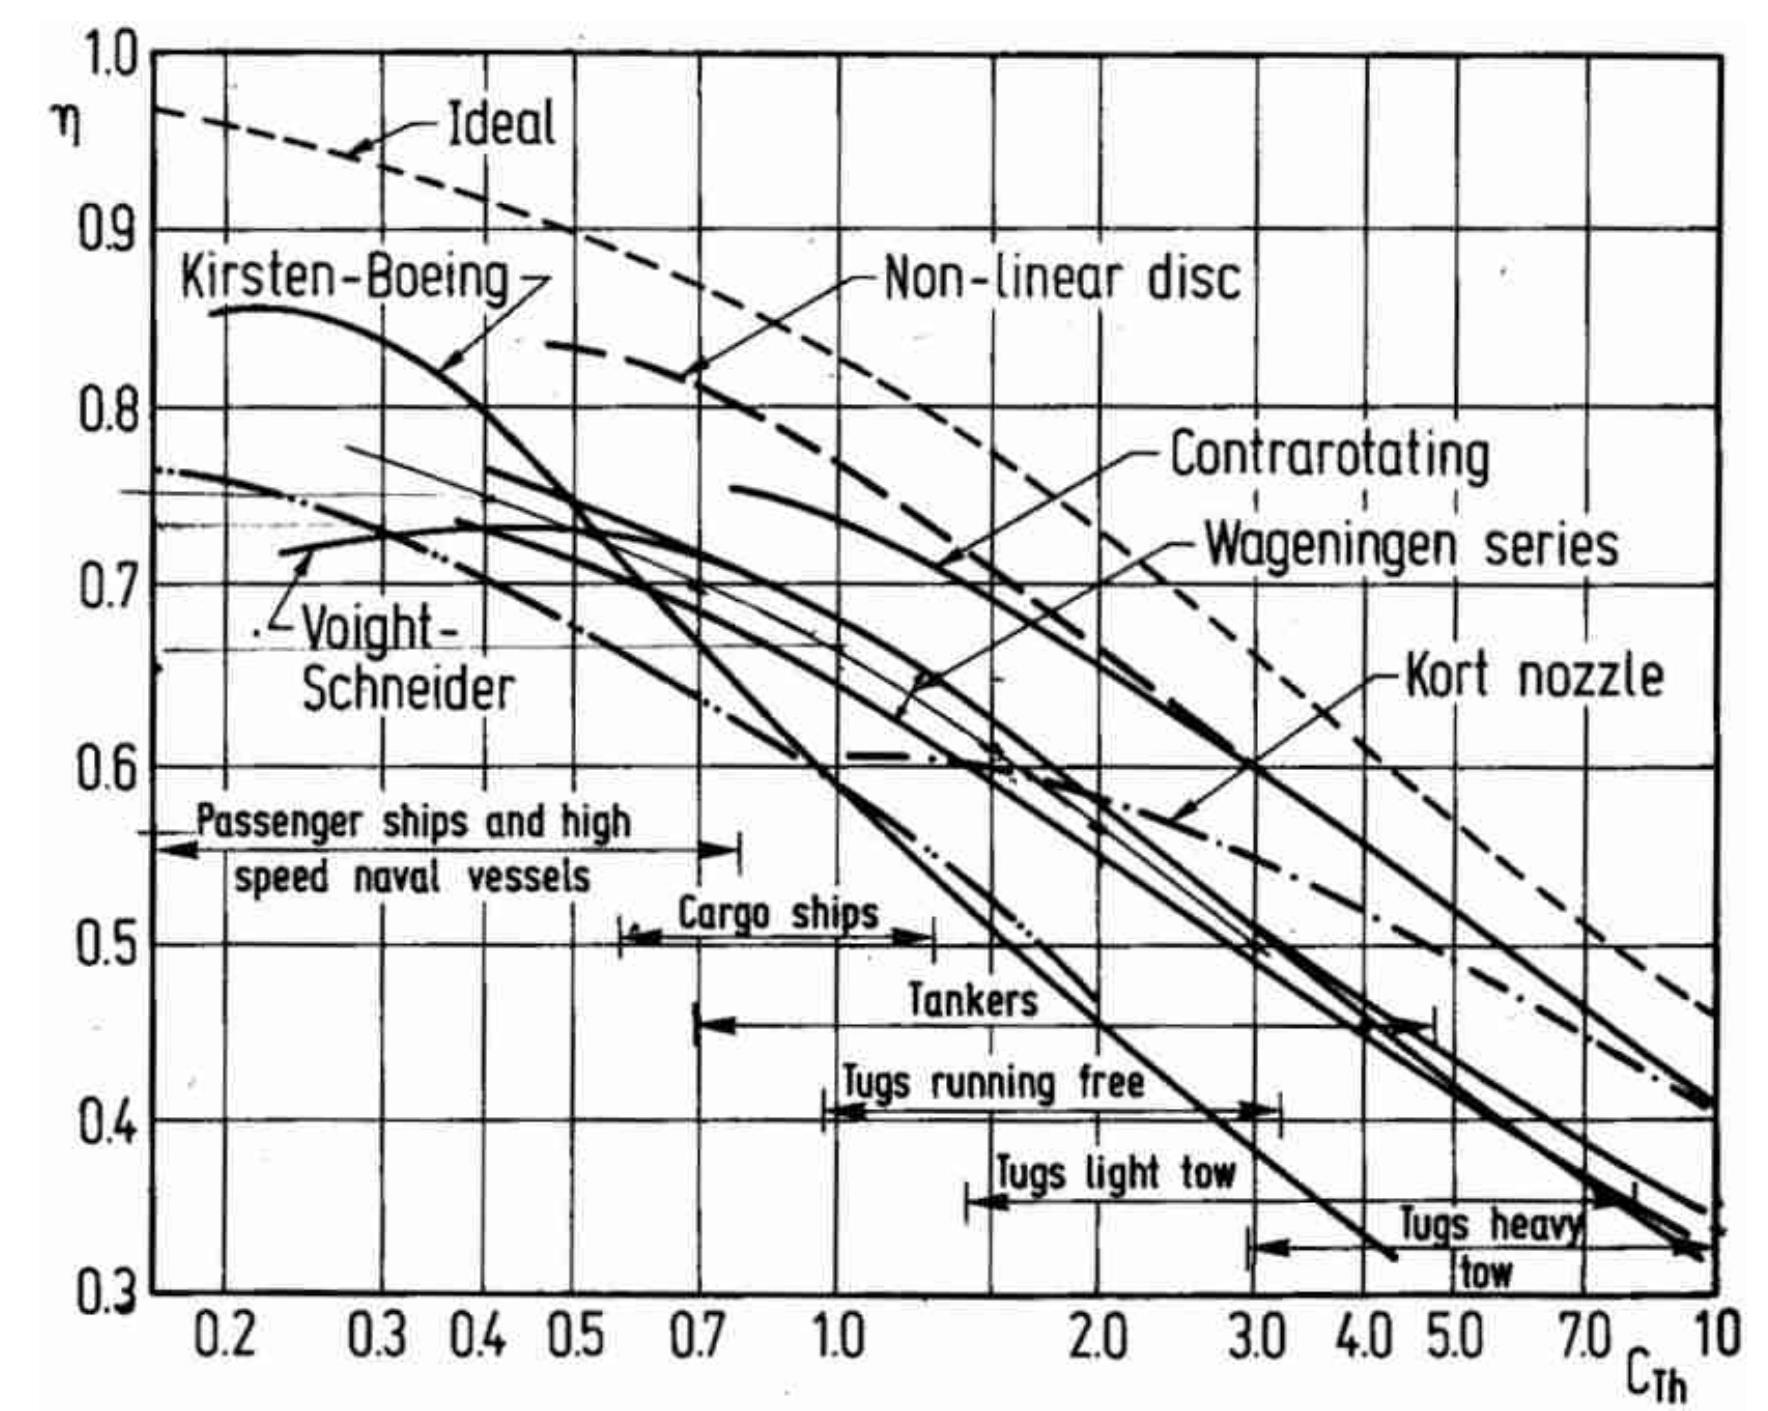
\includegraphics[width=.8\textwidth]{02_figures/Breslin94_openwater_eff.jpg}
        \caption{Efficiencies of various propulsion devices \bcitep{Breslin.1994}}
        \label{fig:breslin_open water efficiencies}
\end{figure}


\subsubsection*{Hull efficiency}

The Hull efficiency $\eta_H$ can be calculated using the following equation:

\begin{equation}
    \label{eqn:hull_eff}
    \eta_H = \frac{1 - t}{1 - w_S}
\end{equation}

The term $t$ refers to the thrust deduction fraction, which represents the thrust force required to overcome the towing resistance of the ship $R_{TOTAL}$ and the additional resistance caused by the propeller's interaction with the hull. On the other hand, the term $w_S$ corresponds to the wake fraction, characterising the influence of the ship's hull on the water flow into the propeller \bcitep{Diesel.2011,Birk.2019}. The following equations are presented for twin-screw vessels\footnote{Considering the length of the equations, the equations for single screw vessels can be obtained from \bcitet{Holtrop.1982} and \bcitet{Birk.2019}} to calculate $w_S$ and $t$.

\begin{equation}
    \label{eqn:wake_ws}
    w_S = 0.3095 C_B + 10 C_V C_B -0.23 \frac{D}{\sqrt{BT}}
\end{equation}

\begin{equation}
    \label{eqn:thrust_t}
    t = 0.325 C_B - 0.1885 \frac{D}{\sqrt{BT}}
\end{equation}

where $C_V$ is the viscous resistance coefficient, which combines all friction-related components of the resistance and the correlation resistance:

\begin{equation}
    \label{eqn:C_V}
    C_V = \frac{(1+k_1)R_F+R_{APP}+R_A}{\frac{1}{2}\rho v_S^2 (S+\sum_i S_{APP_i})}
\end{equation}

\subsubsection*{Relative rotative efficiency}

The relative rotative efficiency \begin{math} \eta_R \end{math} can be expressed by the following ratio, with $v_A$ defined as the arriving water velocity to propeller \bcitep{Diesel.2011}:

\begin{equation}
    \label{eqn: n_rot_MAN}
    \eta_R = \frac{\text{Power absorbed in open water at }v_A}{\text{Power absorbed in wake behind the ship at }v_A}
\end{equation}

According to \bcitet{Holtrop.1982}, $\eta_R$ for twin screw vessels can be estimated using the following formula, with $P/D$ defined as the propeller pitch-to-diameter ratio:

\begin{equation}
    \label{eqn: eta_rot_holtrop}
    \eta_R = 0.9737 + 0.111(C_P-0.0225\ell_{CB}) - 0.06325\frac{P}{D}
\end{equation}

\subsubsection*{Shaft efficiency}

The shaft efficiency \begin{math}\eta_S\end{math} is defined as the ratio between the power delivered to the propeller $P_D$ and the brake power of the main engine $P_B$, with values ranging from $\eta_S = 0.95 - 0.99$ depending on shaft design and gear configuration.


% \begin{tikzpicture}[x=0.75pt,y=0.75pt,yscale=-1,xscale=1]
%     %uncomment if require: \path (0,452); %set diagram left start at 0, and has height of 452
    
%     %Shape: Axis 2D [id:dp697661158302031] 
%     \draw  (220,297.8) -- (517.5,297.8)(249.75,80) -- (249.75,322) (510.5,292.8) -- (517.5,297.8) -- (510.5,302.8) (244.75,87) -- (249.75,80) -- (254.75,87)  ;
%     %Image [id:dp23308396965327827] 
%     \draw (245,305) node [rotate=-40.58] {
\includegraphics[width=26.87pt,height=72.39pt]{02_figures/ferry.jpg}};
% \end{tikzpicture}




% \subsection{Ship speed}


% \subsection{Modelling}



% Phased out, but might be useful

% Might be useful for multiple images !
% \begin{figure}[h]
% \centering
% \begin{minipage}[t]{.5\textwidth}
%     \centering
%     % \begin{figure}
%     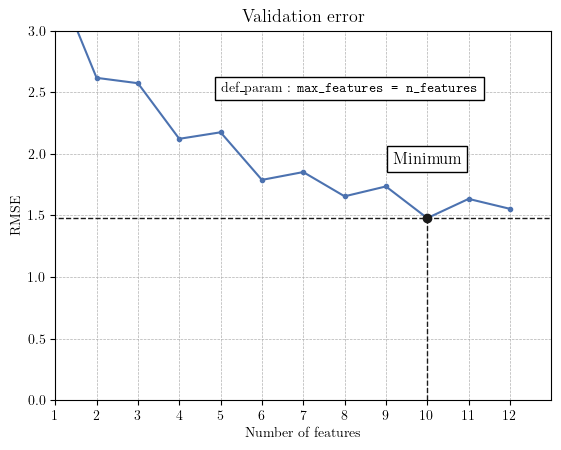
\includegraphics[width=\textwidth]{02_figures/featureserrro.png}
%     % \end{figure}
%     \captionof{figure}{Effects of number of features on RMSE}
%     \label{fig:featureserror}
% \end{minipage}%
% \begin{minipage}[t]{.5\textwidth}
%     \centering
%     % \begin{figure}
%     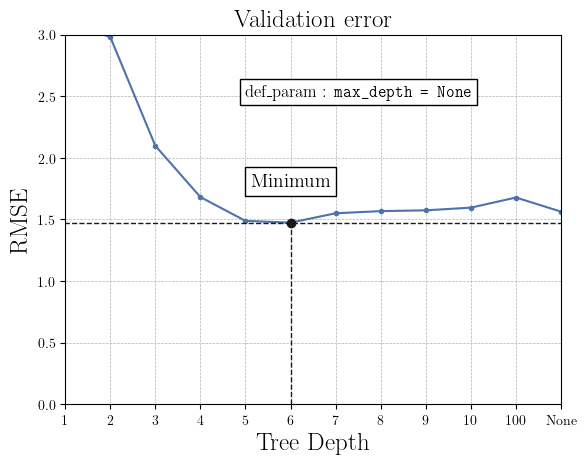
\includegraphics[width=\textwidth]{02_figures/depthError.png}
%     % \end{figure}
%     \captionof{figure}{Effects of tree depth on RMSE}
%     \label{fig:deptherror}
% \end{minipage}
% \end{figure}

% \begin{figure}[h]
%     \centering
%         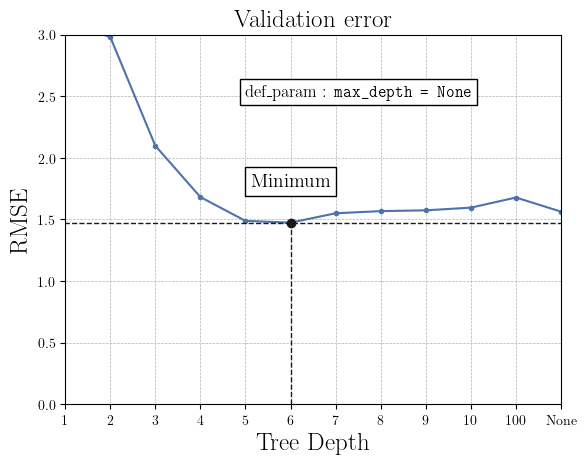
\includegraphics[width=.5\textwidth]{02_figures/depthError.png}
%         \caption{Effect of tree depth on RMSE for validation dataset}
%         \label{fig:Tree Depth Error}
% \end{figure}

% \begin{enumerate}
%     \item Possible thresholds are determined by calculating the splitting value (For example, suppose there are data points at $X = [0.2,0.4]$, then the splitting value is the value in between i.e. $t_k = 0.3$)
%     \item Calculate the mean of data points of the left and right partition space respectively, Defined by the following equation $\hat{y}_{node} = \frac{1}{m_{node}}\sum\limits_{i\in node} y ^ {(i)}$
%     \item Calculate the mean squared error (MSE) of each data points in its respective partition space. Through the equation $MSE_{node} = \sum\limits_{i\in node}(\hat{y}_{node} - y^{(i)} )^2$ 
%     \item The MSE from the respective partition space is summed.
%     \item Step $1 - 4$ is recursively repeated, until the minimum of the cost function $J(X,T_k)$, i.e. minimum MSE, is determined:
%      \begin{equation}\label{costfun}
%         J(X,t_k) = \frac{m_{left}}{m}MSE_{left} + \frac{m_{right}}{m}MSE_{right}
%         \begin{cases}
%             MSE_{node} = \sum\limits_{i\in node}(\hat{y}_{node} - y^{(i)} )^2 \\
%             \hat{y}_{node} = \frac{1}{m_{node}}\sum\limits_{i\in node} y ^ {(i)}
%         \end{cases}   
%     \end{equation}
% \end{enumerate} 